\documentclass{article}

\usepackage{lmodern}
\usepackage[T1]{fontenc}
\usepackage[utf8]{inputenc}

%% Tools for drafting the manuscript, remove for publication
% Drafting

\usepackage[latexmk]{lwarp}

\usepackage{xcolor,soul}
\usepackage{fullpage}
\usepackage{setspace}
\usepackage{blindtext}
\doublespacing

\definecolor{mwcolor}{HTML}{8af67d}
\definecolor{vgcolor}{HTML}{c88bff} % MPL purple
\definecolor{citecolor}{HTML}{c696f0} % MPL purple


% Tools for leaving todo notes around
\usepackage[colorinlistoftodos]{todonotes}
%% \renewcommand{\todo}{}
%% \renewcommand{\hl}[1]{#1}
\newcommand{\citeme}[1]{%
  \todo[color=citecolor]{%
  \ifstrempty{#1}{[citation needed]}{[cite: #1]}%
  }%
}
\newcommand{\mw}[2]{%
  \sethlcolor{mwcolor}\hl{#2}\sethlcolor{yellow}%
  \ifstrempty{#1}{}{%
    \todo[color=mwcolor]{#1 [MW]}%
  }%                  
}
\newcommand{\vg}[2]{%
  \sethlcolor{vgcolor}\hl{#2}\sethlcolor{yellow}%
  \ifstrempty{#1}{}{%
    \todo[color=vgcolor]{#1 [VG]}%
  }%                  
}


\usepackage{graphicx}
\usepackage{booktabs}  % For making tables look nice
\usepackage[hidelinks]{hyperref}
\usepackage[version=4]{mhchem}
\usepackage{siunitx}
\usepackage[xr,user]{zref} % For cross references to supplement figures
\usepackage{glossaries}
\usepackage{textgreek}

\newcommand{\nca}[1]{\ce{Li_{#1}Ni_{0.8}Co_{0.15}Al_{0.05}O_2}}
\DeclareRobustCommand{\nmc}[2][]{%
    \ifstrempty{#1}{%
        \ce{Li_{#2}Ni_{y}Mn_{z}Co_{1-y-z}O2}}{}%
    \ifstrequal{#1}{333}{%
        \ce{Li_{#2}Ni_{1/3}Mn_{1/3}Co_{1/3}O2}}{}%
    \ifstrequal{#1}{532}{%
        \ce{Li_{#2}Ni_{0.5}Mn_{0.3}Co_{0.2}O2}}{}%
}

%% Define colors
\definecolor{ligreen}{HTML}{63A656}
\definecolor{mnpurple}{HTML}{6E0567}
\definecolor{ored}{HTML}{AB0200}
\definecolor{coblue}{HTML}{000082}
\definecolor{C0}{HTML}{1F77B4}
\definecolor{C1}{HTML}{FF7F0E}
\definecolor{C2}{HTML}{2CA02C}
\definecolor{C3}{HTML}{D62728}
\definecolor{C4}{HTML}{9467BD}
\definecolor{C5}{HTML}{8C564B}
\definecolor{C6}{HTML}{E377C2}
\definecolor{C7}{HTML}{7F7F7F}
\definecolor{C8}{HTML}{BCBD22}
\definecolor{C9}{HTML}{17BECF}

% Techniques
\newacronym{xrd}{PXRD}{powder X-ray diffraction}
\newacronym{uxrd}{µ-XRD}{X-ray microdiffraction}
\newacronym{txm}{TXM}{transmission X-ray microscopy}
\newacronym{xas}{XAS}{X-ray absorbance spectroscopy}
\newacronym{xanes}{XANES}{X-ray absorbance near edge spectroscopy}
\newacronym{iscat}{iSCAT}{optical interferometric scattering microscopy}

% Facilities and organizations
\newacronym{ssrl}{SSRL}{Stanford Synchrotron Radiation Lightsource}

% Chemistry
%\newacronym{ecd}{ECD}{exchange current density}
\newacronym{ecd}{$i_0$}{exchange current density}
\newacronym{od}{OD}{optical depth}
\newacronym{ocv}{OCV}{open circuit voltage}

% Particles in u-XRD mapping
\newacronym{p1}{P1}{particle 1}
\newacronym{p2}{P2}{particle 2}
\newacronym{p3}{P3}{particle 3}



\usepackage{authblk}

\title{Origin of Rapid Delithiation In Secondary Particles Of \nca{} and \nmc{} Cathodes}

\author[1,2,3]{Mark Wolfman}
\author[1]{Brian M.\ May}
\author[4]{Vishwas Goel}
\author[4]{Sicen Du}
\author[5,6]{Young-Sang Yu}
\author[7]{Nicholas V.\ Faenza}
\author[7]{Nathalie Pereira}
\author[8]{Antonin Grenier}
\author[3]{Kamila M.\ Wiaderek}
\author[3]{Ruqing Xu}
\author[9]{Jiajun Wang}
\author[8]{Karena W.\ Chapman}
\author[7]{Glenn G.\ Amatucci}
\author[4]{Katsuyo Thornton}
\author[1]{Jordi Cabana\thanks{Corresponding author: jcabana@uic.edu}}

\affil[1]{Department of Chemistry, University of Illinois at Chicago}
\affil[2]{Chemical Sciences and Engineering Division, Argonne National Laboratory}
\affil[3]{X-ray Science Division, Advanced Photon Source, Argonne National Laboratory}
\affil[4]{Department of Materials Science and Engineering, University of Michigan}
\affil[5]{Department of Physics, Chungbuk National University}
\affil[6]{Advanced Light Source, Lawrence Berkeley National Laboratory}
\affil[7]{Energy Storage Research Group, Department of Materials Science and Engineering, Rutgers, The State University of New Jersey}
\affil[8]{Department of Chemistry, Stony Brook University}
\affil[9]{Harbin Institute of Technology}

\date{}

\makeatletter
\let\mytitle\@title
\title{Supplemental Information: \mytitle}
\makeatother

% Make figures show up as "S1" etc.
\renewcommand{\thefigure}{S\arabic{figure}}
\renewcommand{\thetable}{S\arabic{table}}

\graphicspath{{./figures/}}

\begin{document}

\maketitle


\section{Model Equations}

\subsection{8-Particle Ensemble}

The cell used in our 8-particle simulations consists of a Li metal
anode and an \nca{} cathode, which contains 8 particles ranging from
\SIrange{2}{5.5}{\micro\meter} in radius, as shown in the Figure
\ref{fig:8-particle-box}. All the particles are attached to a metallic
current collector, which is also shown in Figure
\ref{fig:8-particle-box}. The two electrodes are separated by a pool
of electrolyte. The size of the computational domain is $50\times
50\times 50$ \si{\micro\meter\cubed}.

\begin{figure}
  \centering
  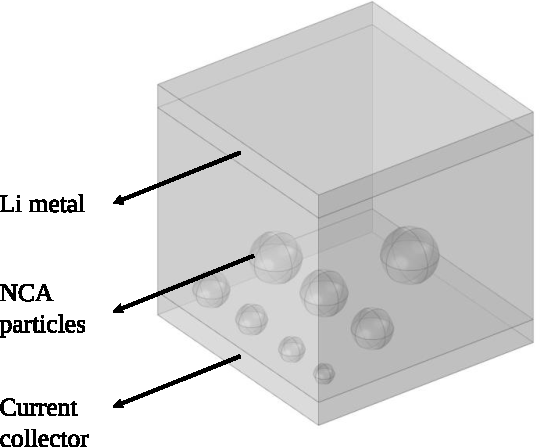
\includegraphics[width=0.5\textwidth]{8-particle-simulation.pdf}
  \caption{The 8-particle simulation setup in COMSOL.}
  \label{fig:8-particle-box}
\end{figure}

Within the \nca{} particles, the mass transport is calculated
as\cite{newman1993,newman1994}

\begin{equation}
  \frac{\partial c_{p,k}}{\partial t}=\frac 1{r^2}\frac \partial {\partial r}\left(D_pr^2\frac{\partial c_{p,k}}{\partial r}\right)
  \label{eq:1a}
\end{equation}
  
where $c_p$ is the \gls{xLi} in the electrode particles, $t$ is time,
$r$ is the radial distance, $D_p$ is the Li diffusivity in \nca{}. The
subscript $k$ represents the particle number from hereon.

The boundary conditions for Equation \ref{eq:1a} are as
follows\cite{newman1993,newman1994}

\begin{subequations}
    \begin{align}
      -D_p\frac{\partial c_{p,k}}{\partial r}|_{r=R_{p,k}} &= J_{k} \label{eq:1b} \\
      -D_p\frac{\partial c_{p,k}}{\partial r}|_{r=0} &= 0 \label{eq:1c}
    \end{align}
\end{subequations}

where $R_{p,k}$ represents the particle radius. Furthermore, all the
particles are set to have an initial \gls{xLi} of $c_p^0$.

The electrochemical reaction flux ($J_k$) at the \nca{}/electrolyte
interface for each particle is calculated using the Butler-Volmer
equation as\cite{newman1993,newman1994}

\begin{subequations}
\begin{equation}
  J_k = \frac{i_0}{F}\times\left(\exp \left(\frac{0.5F}{RT}\eta{}_k\right)-\exp
  \left(\frac{-0.5F}{RT}\eta{}_k\right)\right)
  \label{eq:2a}
\end{equation}
\begin{equation}
  \eta{}_k=\phi{}_{p,k}-\phi{}_e-U_k^0
  \label{eq:2b}
\end{equation}
\end{subequations}

where $i_0$ is the exchange current density, $F$ is the Faraday
constant, $R$ is the ideal gas constant, $T$ is absolute temperature,
$\eta{}_k$ is overpotential on the surface of $k^{\mathit{th}}$
particle. Furthermore, $\phi{}_{p,k}$ is the electrostatic potential of the
particle, $\phi{}_e$ is the electrostatic potential of the electrolyte, and
$U_k^0$ is the \gls{ocv} of \nca{} vs.\ce{Li/Li^+}.

The electrostatic potential of \nca{} particles is obtained as\cite{newman1993,newman1994}

\begin{equation}
  -\sigma{}_p\nabla{}\phi{}_{p,k}=i_{p,k}
  \label{eq:3}
\end{equation}

where $\sigma{}_p$ is the electronic conductivity of \nca{} and $i_{p,k}$ is
the current density on the $k^{\mathit{th}}$ particle. It should be
noted that $i_{p,k}=J_kF$.

The electrochemical reaction flux and the electrostatic potential at
the Li metal anode is calculated in a similar manner as Equations
\ref{eq:2a}--\ref{eq:3} as\cite{dasgupta2016}

\begin{subequations}
\begin{equation}
  J_{\mathrm{Li}}=\frac{i'_0}{F}\times \left(\exp\left(\frac{0.5F}{RT}\eta{}_{\mathrm{Li}}\right)-\exp\left(\frac{-0.5F}{RT}\eta{}_{\mathrm{Li}}\right)\right)
  \label{eq:4a}
\end{equation}
\begin{equation}
  \eta{}_{\mathrm{Li}}=\phi{}_{\mathrm{Li}}-\phi{}_e-U_{\mathrm{Li}}^0
  \label{eq:4b}
\end{equation}
\end{subequations}

where $J_{\mathrm{Li}}$, $i'_0$, and $\eta{}_{\mathrm{Li}}$ are the
reaction flux, the exchange current density, and the overpotential at
the Li metal anode/electrolyte interface, respectively. The
electrostatic potential and the \gls{ocv} of the electrode are given
by $\phi{}_{\mathrm{Li}}$ and $U_{\mathrm{Li}}^0$,
respectively. Furthermore, $\phi{}_{\mathrm{Li}}$ is obtained
as\cite{newman1993,newman1994}

\begin{equation}
  -\sigma{}_{\mathrm{Li}}\nabla{}\phi{}_{\mathrm{Li}}=i_{\mathrm{app}}
  \label{eq:5}
\end{equation}

where $\sigma{}_{\mathrm{Li}}$ is the electronic conductivity of Li metal and
$i_{\mathrm{app}}$ is the applied current density to the cell. It
should be noted that
$\sum_k4\pi R_{p,k}^2i_{p,k}=i_{\mathrm{app}}A$, where $A$ is the
cross-sectional area of both the current collector (in contact with
the \nca{} cathode) and the Li metal anode. Moreover, we set the top
surface of the Li metal anode as ground.

The mass transport equation for the electrolyte is written as\cite{newman1993,newman1994}

\begin{equation}
  \frac{\partial c_e}{\partial t} = \nabla \cdot \left(D_e \nabla c_e \right) - \frac{i_e\cdot\nabla{}t_{+}^0}{F}
  \label{eq:6}
\end{equation}

where $D_e$ represents the electrolyte diffusivity, $i_e$ represents
the electrolyte current density, and $t_+^0$ represents the
transference number for \ce{Li^+}. The initial value of $c_e$ is set
as $c_e^0$. Finally, $i_e$ is calculated as\cite{newman1993,newman1994}

\begin{equation}
  i_e=-\sigma_e\nabla \phi _e+\frac{2RT}{F}\sigma_e\left(1+\frac{\partial \ln \left(f_{\pm}\right)}{\partial \ln \left(c_e\right)}\right)\left(1-t_+^0\right)\nabla \ln c_e
  \label{eq:7}
\end{equation}

where $\sigma_e$ is the electrolyte conductivity and $\frac{\partial
  \ln \left(f_\pm\right)}{\partial \ln \left(c_e\right)}$ accounts for
the salt activity coefficient dependence on the electrolyte
concentration.

\subsection{30-Particle Ensemble}

For the 30-particle system, we only solve for the diffusion of Li in
NCA particles (Equations \ref{eq:1a}--\ref{eq:1c}) and the
electrochemical reaction at the \nca{}/electrolyte interface
(Equations \ref{eq:2a} and \ref{eq:2b}). We do not solve for the
electrostatic potentials in \nca{} particles (Equation \ref{eq:5}) and
the electrolyte (Equation \ref{eq:7}) and the electrolyte
concentration (Equation \ref{eq:6}) because the applied C-rate (C/20)
is too low to cause any significant spatial variations in them. Thus,
we assume these potentials to be constant.  Furthermore, we do not
include the Li-metal anode (Equations \ref{eq:3},
\ref{eq:4a}--\ref{eq:4b}) because it does not offer any significant
overpotential during C/20 charging.

We reformulate Equations \ref{eq:1a} and \ref{eq:2b} to a form suitable
for the smoothed boundary method\cite{thornton2012,thornton2018}. The
reformulated form is written as\cite{thornton2018}

\begin{equation}
  \frac{\partial c_{p,k}}{\partial t}=\frac 1{\psi{}_k}\nabla \cdot \psi{}_kD_p\nabla c_{p,k}+\frac{\left|\nabla \psi{}_k\right|}{\psi{}_k}J_k
  \label{eq:8}
\end{equation}

where $\psi{}_k$ \ represents a continuous domain parameter that a value of
1 within the $k^{\mathit{th}}$ particle and 0 outside the
particle. The particle/electrolyte interface is defined as the region
where $ 0 < \psi{}_k < 1 $.


\section{Numerical implementation of the model equations}

\subsection{8-Particle Ensemble}

The system of coupled partial differential equations listed above was
solved in COMSOL Multiphysics 5.6a using the finite element method. A
custom mesh with linear tetrahedral elements was used to discretize
the model geometry. The maximum and minimum element sizes within the
\nca{} particles were set to \num{6.5e-7} and \num{1e-8},
respectively. The model was solved using the multifrontal massively
parallel sparse direct solver \cite{lexcellent2000} and a backward differential
formula solver for time-stepping with a relative tolerance of
\num{1e-5}.

\subsection{30-Particle Ensemble}

The system of coupled governing equation listed above was solved by
the finite difference method. The computational domain is discretized
by a 3D uniform cartesian grid with a spatial resolution of $\Delta
x=\Delta y=\Delta z= \SI{0.1}{\micro\meter}$. We set the time-stepping
as \SI{0.02}{\second} and the relative tolerance for the applied
current during each time step is \num{1e-4}.


\section{Configuration of Particles in the 30-Particle Ensemble}

The particle sizes of the \nca{} powders are D10:
\SI{3.7}{\micro\meter}, D50: \SI{6.5}{\micro\meter}, and D90:
\SI{9.8}{\micro\meter}. We assume a log-normal distribution to
describe the particle size distribution:

\begin{subequations}
\begin{align}
  f(x) & = \frac {1}{\sqrt{2\pi}\sigma x} \exp \left(-\frac{(\ln{x}-\mu )^2}{2\sigma^2}\right)
  \label{eq:10a} \\
  F(x) &= \frac{1}{2} \mathrm{efrc}\left(-\frac{\ln{x}-\mu }{\sqrt{2}\sigma}\right)
  \label{eq:10b}
\end{align}
\end{subequations}

where $x$ is the random variable satisfying a log-normal distribution,
$f(x)$ is the probability density function of $x$, $\sigma$ is the
standard deviation of $x$, $\mu$ is the mean of $x$, $F(x)$ is the
cumulative density function of $x$, and $\mathrm{efrc}$ is the
complementary error function.

We fit these three cumulative distribution values with Equation
\ref{eq:10b}, which yields $\mu =1.8718$, $\sigma=0.1027$. To maintain
the statistics of the real particle size distribution, we use the
stratified sampling\cite{parsons2017} with sampling particle diameter
systematically within each stratum. After determining the particle
size distribution, we randomly generate the centers of these particles
and use a hyperbolic tangent function to generate the domain
parameters for individual particle, $\psi{}_k$:

\begin{equation}
  \psi_k=\frac{1}{2}+\frac{1}{2}\tanh\left(\frac{r-d}{\delta}\right)
  \label{eq:11}
\end{equation}

where $r$ is the radius of this particle, $d$ is the distance to the
particle center, $\delta$ determines the interfacial thickness and we
used $\delta = \sqrt{2}$.

Figure \ref{fig:30-particle-box} shows the particle size distributions
obtained by stratified sampling\cite{parsons2017} and the
computational domain for the 30-particle simulations.

\begin{figure}
  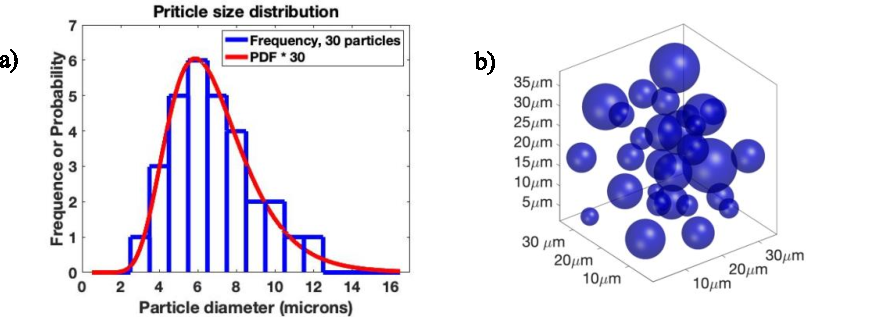
\includegraphics[width=\textwidth]{30-particle-simulation.pdf}
  \caption{(a) The size distribution in the 30-particle system. (b) The
    computational domain for the 30-particle system. The domain has a
    size of $36 \times 36 \times 40$ \si{\micro\meter\cubed} ($360
    \times 360 \times 400$ grid points).}
  \label{fig:30-particle-box}
\end{figure}

\section{Model Parameters}

\subsection{Open Circuit Voltage}

\begin{figure}
  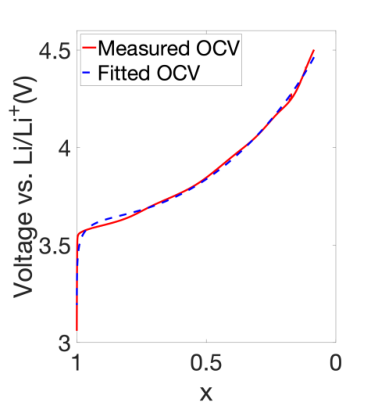
\includegraphics[width=0.5\textwidth]{echem-fit.pdf}
  \caption{Parameterized fitting of \gls{ocv} response. Red line
    denotes the measured \gls{ocv} curve, the blue line denotes the
    fitted \gls{ocv} curve.}
  \label{fig:ocv-response}
\end{figure}

The \gls{ocv} was measured for the 1st charge of Toda \nca{} at
\SI{0.02}{\per\hour} (C/50, Figure \ref{fig:ocv-response}). The
procedure of measurements can be found in Liu et al.'s
paper\cite{liu2017}.

We fitted the experimentally measured \gls{ocv} data with the
following equation:

\begin{equation}
  \mathit{OCV}=a\ln \left(\frac x{1-x}\right)+b\left(x-1\right)^2+cx^2+d
  \label{eq:12}
\end{equation}

Where $a=\SI{-0.06809}{\volt}$, $b=\SI{0.9009}{\volt}$,
$c=\SI{0.2749}{\volt}$, $d=\SI{3.544}{\volt}$. $x$ represents the
lithium fraction.

\subsection{Li Diffusivity in \nca{}}

\begin{figure}
  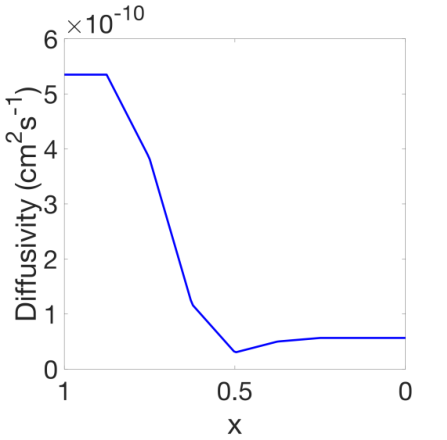
\includegraphics[width=0.5\textwidth]{diffusivity.pdf}
  \caption{$D_s$ as a function of $x$ for the \nca{} material\cite{amin2015}.}
  \label{fig:diffusivity}
\end{figure}

The diffusivity values are obtained from the report by Amin et
al\cite{amin2015}. We use linear interpolation to estimate the
diffusivity values between data points. For the regions close to
fully delithiation and fully lithiation, we set the diffusivity values
the same as the closest data point.

\subsection{Electrolyte Parameters}

Like our previous works\cite{dasgupta2020,dasgupta2020-2}, all the electrolyte parameters,
namely $\sigma_e$, $D_e$, $\frac{\partial \ln
  \left(f_\pm\right)}{\partial \ln \left(c_e\right)}$, and $t_+^0$ are
obtained from the report by Nyman et al\cite{lindbergh2008}.


\subsection{Remaining Parameters}

The remaining model parameters are described in Table \ref{tab:model-parameters}.

\begin{table}
  \begin{tabular}{r | l l l}
    \hline
    Parameters & Values & Units & Source \\
    \hline\hline
    Electronic conductivity of NCA + carbon additive, $\sigma_p$ & \num{9.1e1} & \si{\siemens\per\meter} & Literature\cite{lindbergh2008-2} \\
    Electronic conductivity of Li, $\sigma_{\mathrm{Li}}$ & \num{1e5} & \si{\siemens\per\meter} & --  \\
    Exchange current density of Li, $i'_0$ & \num{9.65e1} & \si{\ampere\per\meter\squared} & Literature \cite{moshtev1984} \\
    \gls{ocv} of Li metal, $U_{\mathrm{Li}}^0$ & 0 & \si{\volt} & -- \\
    Max \gls{xLi} in NCA, $c_p^{\mathrm{max}}$ & \num{4.8e4} & \si{\mole\per\meter\cubed} & Estimated based on literature \cite{sauer2015,bund2018,sauer2018} \\
    Initial \gls{xLi} in NCA, $c_p^0$ & $0.99\times c_p^{\mathrm{max}}$ & \si{\mole\per\meter\cubed} & Presumed \\
    Initial electrolyte salt concentration, $c_e^0$ & \num{1e3} & \si{\mole\per\meter\cubed} & Experiment \\
    Temperature & \num{2.98e2} & \si{\kelvin} & Experiment \\
    1C current density & \num{1.164} & \si{\ampere\per\meter\squared} & Experiment \\
    \hline
  \end{tabular}
  \caption{Additional parameters used in physics modeling.}
  \label{tab:model-parameters}
\end{table}
 


\section{Sensitivity Analyses with Respect to \Gls{ecd}}

In this section, we report the results of the sensitivity studies with
respect to different forms of \gls{ecd}. We note that we set $D_s>
\SI{5e-15}{\meter\squared\per\second}$ (as shown in Figure
\ref{fig:diffusivity}) for all simulations in this section to avoid
solid-state limitation in the simulated system.


\section{Selection of $i_0$ Function}

Traditionally, $i_0$ is considered to be directly proportional to
$\sqrt{x\left(1-x\right)}$, where $x$ is the Li site fraction in the
active
material\cite{newman1993,newman1994-2,newman1995-2,newman1996}. This
functional form results from the theoretical consideration that Li
exists in a solid solution state in the active material. However,
recent studies have shown that such a dependence is not applicable for
materials like \nca{}\cite{chueh2021} and \nmc{}\cite{mukherjee2017,chiang2020,tsai2018}. For
example, Park et al.\cite{chueh2021}\ reported an exponential
dependence of $i_0$ on $x$\cite{chueh2021}. Other studies show that
$i_0$ is a monotonically decreasing function of
$x$\cite{mukherjee2017,chiang2020,tsai2018}. Thus, the dependence of $i_0$ on $x$ is not
precisely known. Furthermore, the literature is missing the $i_0$ data
for $x>0.92$.

To work with the uncertain form of $i_0$, we ran two sets of
simulations. In the first set of the simulations, we employed the
traditional form of $i_0$, which is shown in Figure \ref{fig:i0_profiles}. In
the second set of simulations, we used a model form of $i_0$, which is
also shown in Figure \ref{fig:i0_profiles}. The model form is setup to have a
smooth step function of $x$; the step in the function is described by
a cubic spline.

\begin{figure}
  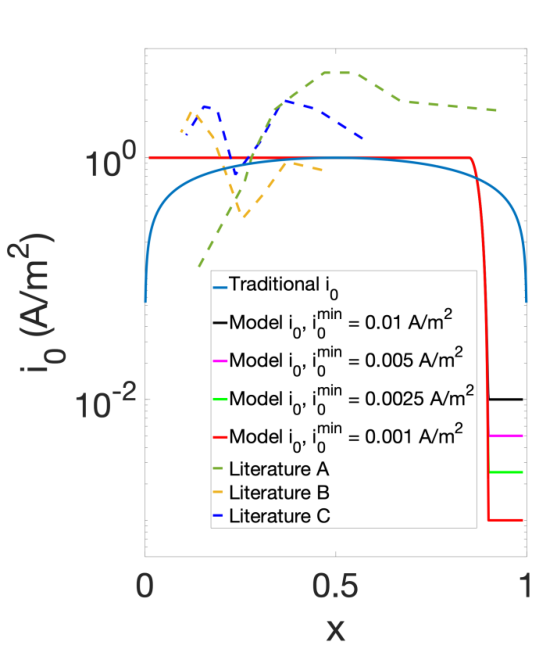
\includegraphics[width=0.5\textwidth]{i0_sensitivity.pdf}
  \caption{Log scale comparison of different \gls{ecd} functions used
    in the sensitivity analyses. The literature-reported functions are
    shown in dashed lines.  The plot labeled as ``Literature A'' is
    obtained from Reference\cite{dees2008}, whereas the plots labeled
    as ``Literature B'' and ``Literature C'' are obtained from
    Reference \cite{tsai2018}.}
  \label{fig:i0_profiles}
\end{figure}

The traditional form only has the max value of $i_0$,
$i_0^{\mathrm{max}}$, as a tunable parameter, whereas the model form
has four parameters: \ $i_0^{\mathrm{min}}$, the minimum value of
$i_0$; $i_0^{\mathrm{max}}$; $x^{\ast }$, the value of $x$ \ where the
transition begins from $i_0^{\mathrm{min}}$ \ to $i_0^{\mathrm{max}}$;
and $\Delta x$, the width of the transition zone. The presence of additional
parameters enables the model function of $i_0$ \ to represent most of
the aforementioned-literature-reported functions. Since the values of
$i_0^{\mathrm{max}}$ \ reported in the %
%Need to add one more reference here. I need to confirm it with Sicen. 
%Goel, Vishwas
%September 27, 2021, 9:03 PM
literature\cite{tsai2018,dees2008} \ do not vary widely, we selected
an intermediate value,
$i_0^{\mathrm{max}}=\SI{1}{\ampere\per\meter\squared}$. The comparison
of the literature values with the traditional and model functions of
$i_0$ \ is provided in Figure \ref{fig:i0_profiles}.

\section{Effect of $i_0$ on the Delithiation Dynamics}

The evolution of the volume average Li-site fraction, $\left\langle
x\right\rangle $, for the first set of simulations, i.e., with the
traditional form of $i_0$ at \SI{0.05}{\per\hour} (C/20) are provided
in Figure \ref{fig:x-evolution}. All the particles delithiate at the
same uniform rate. For the second set of simulations using the model
form of $i_0$, the evolution results will be presented individually
for the sensitivity analyses with respect to $i_0^{\mathrm{min}}$,
$x^{\ast}$, and $\Delta x$.

\begin{figure}
  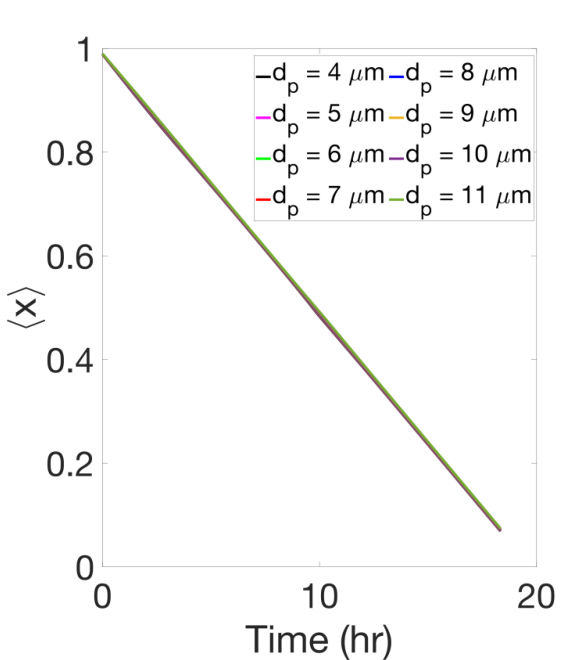
\includegraphics[width=0.5\textwidth]{8-particle-evolution.pdf}
  \caption{Evolution of $\langle x \rangle$ for the 8-particle system
    obtained using the traditional function of \gls{ecd}. All the
    particles delithiate at the same rate.}
  \label{fig:x-evolution}
\end{figure}

\section{Sensitivity Analyses with Respect to $i_0^{\mathrm{min}}$}

We chose four different values of $i_0^{\mathrm{min}}$ ranging from
\SIrange{0.001}{0.01}{\ampere\per\meter\squared}, while setting the
value of other parameters as
$i_0^{\mathrm{max}}=\SI{1}{\ampere\per\meter\squared}$, $x^{\ast
}=0.9$, and $\Delta x=0.05$. The comparison of different $i_0$
functions that differ in terms of $i_0^{\mathrm{min}}$ is provided in
Figure \ref{fig:i0_profiles}. The corresponding results for the
evolution of $\left\langle x\right\rangle $ are provided in Figure
\ref{fig:i0-sensitivity}. All particles exhibit accelerated
delithiation for all values of $i_0^{\mathrm{min}}$. Furthermore, as
$i_0^{\mathrm{min}}$ is decreased, the $\left\langle x\right\rangle $
value at which the accelerated delithiation of each particle halts
also decreases, which will hereafter be denoted as $\left\langle
x\right\rangle^\dag$. Since the $i_0^{\mathrm{min}}$ value of
\SI{0.001}{\ampere\per\meter\squared} resulted in a similar value of
$\left\langle x\right\rangle^\dag$ as the experiments, we selected
this $i_0^{\mathrm{min}}$ value as the nominal value. As explained in
the main text, the oscillations in $\left\langle x\right\rangle $ in a
few cases originate because of the large difference between
$i_0^{\mathrm{min}}$ and $i_0^{\mathrm{max}}$.

\begin{figure}
  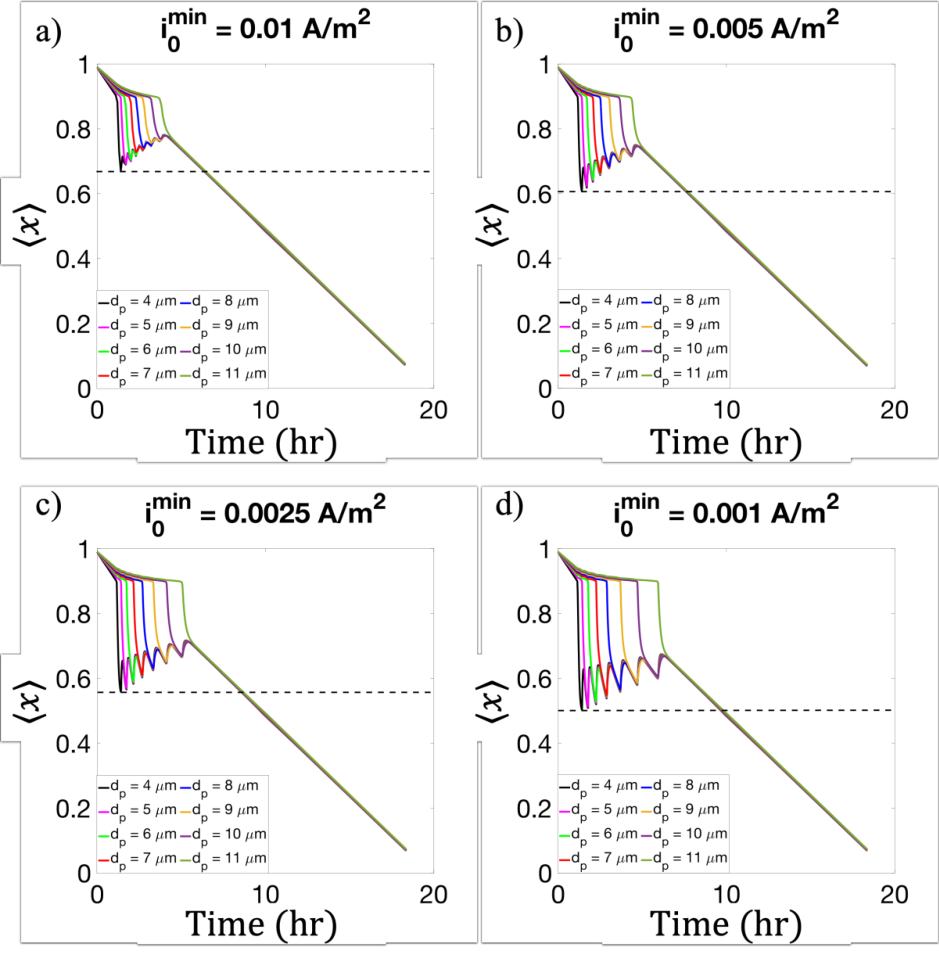
\includegraphics[width=\textwidth]{8-particle-evolution-i0min.pdf}
  \caption{Evolution of $\langle x \rangle$ for the 8-particle system obtained using
    the model form of \gls{ecd} with four different values of
    $i_0^{\mathrm{min}}$: a) \SI{0.01}{\ampere\per\meter\squared}, b)
    \SI{0.005}{\ampere\per\meter\squared}, c)
    \SI{0.0025}{\ampere\per\meter\squared}, and d)
    \SI{0.001}{\ampere\per\meter\squared}. The black dashed line in
    each plot represents $\langle x \rangle^\dag$ for the smallest particle in the
    ensemble; $\langle x \rangle^\dag$ decreases with a decrease in $i_0^{\mathrm{min}}$.}
  \label{fig:i0-sensitivity}
\end{figure}

\section{Sensitivity analyses with respect to $x^{\ast}$}

We choose four different values of $x^{\ast}$ ranging from 0.9 to 0.6,
and we set the parameters as
$i_0^{\mathrm{max}}=\SI{1}{\ampere\per\meter\squared}$,
$i_0^{\mathrm{min}}=\SI{1e-3}{\ampere\per\meter\squared}$, and $\Delta
x=0.05$. Figure \ref{fig:x-star-sensitivity} shows the comparison of
different $x^{\ast }$ values. The onset of the accelerated
delithiation is determined by the $x^\ast$ value and $\langle x
\rangle^\dag$ decreases with a decrease in $x^\ast$.

\begin{figure}
  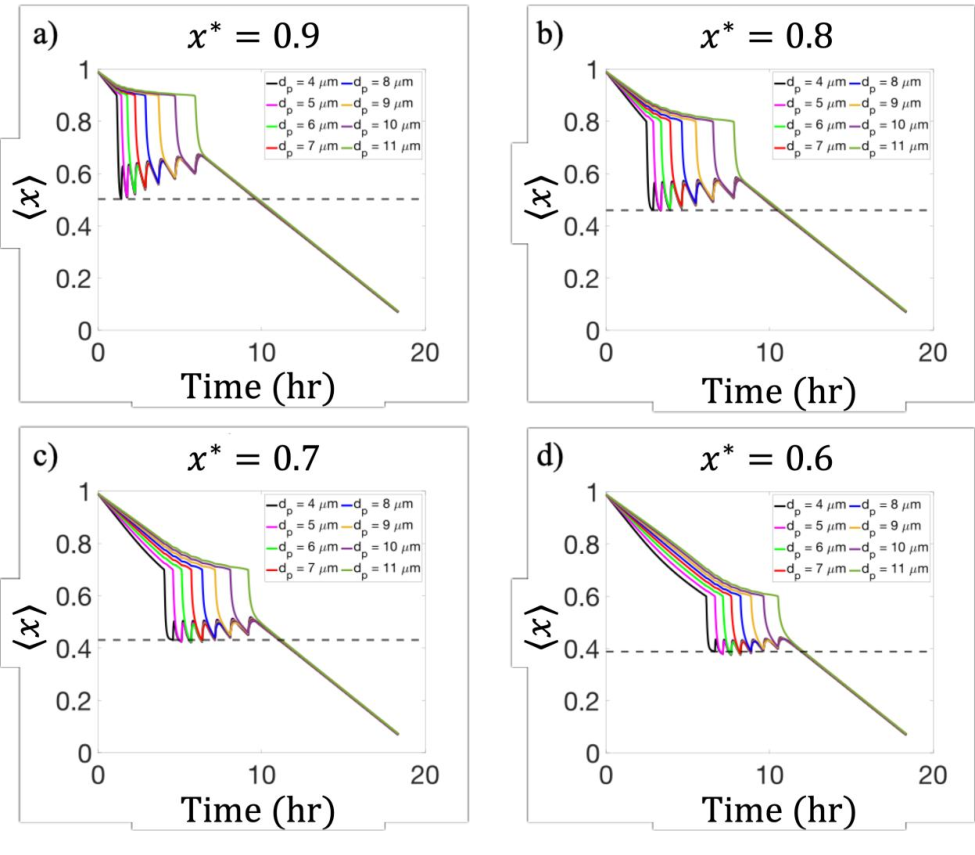
\includegraphics[width=\textwidth]{8-particle-evolution-xstar.pdf}
  \caption{Evolution of $\langle x \rangle$ for the 8-particle system obtained using
    the model form of $i_0$ with four different values of $x^\ast$: a)
    0.9, b) 0.8, c) 0.7, and d) 0.6. The black dashed line in each
    plot represents $\langle x \rangle^\dag$ for the smallest particle in the
    ensemble. Note that $\langle x \rangle^\dag$ decreases with a decrease in
    $x^\ast$.}
  \label{fig:x-star-sensitivity}
\end{figure}

\section{Sensitivity analyses with respect to $\Delta x$}

We choose four different values of $\Delta x$ ranging from 0.05 to
0.8, and we set other parameters as
$i_0^{\mathrm{max}}=\SI{1}{\ampere\per\meter\squared}$,
$i_0^{\mathrm{min}}=\SI{1e-3}{\ampere\per\meter\squared}$, and
$x^\ast=0.9$. Figure \ref{fig:delta-x-sensitivity} shows the comparison of different
$\Delta x$ values. Both the amplitudes of the oscillations and the
rate of accelerated delithiation are reduced as $\Delta x$ is
increased.

\begin{figure}
  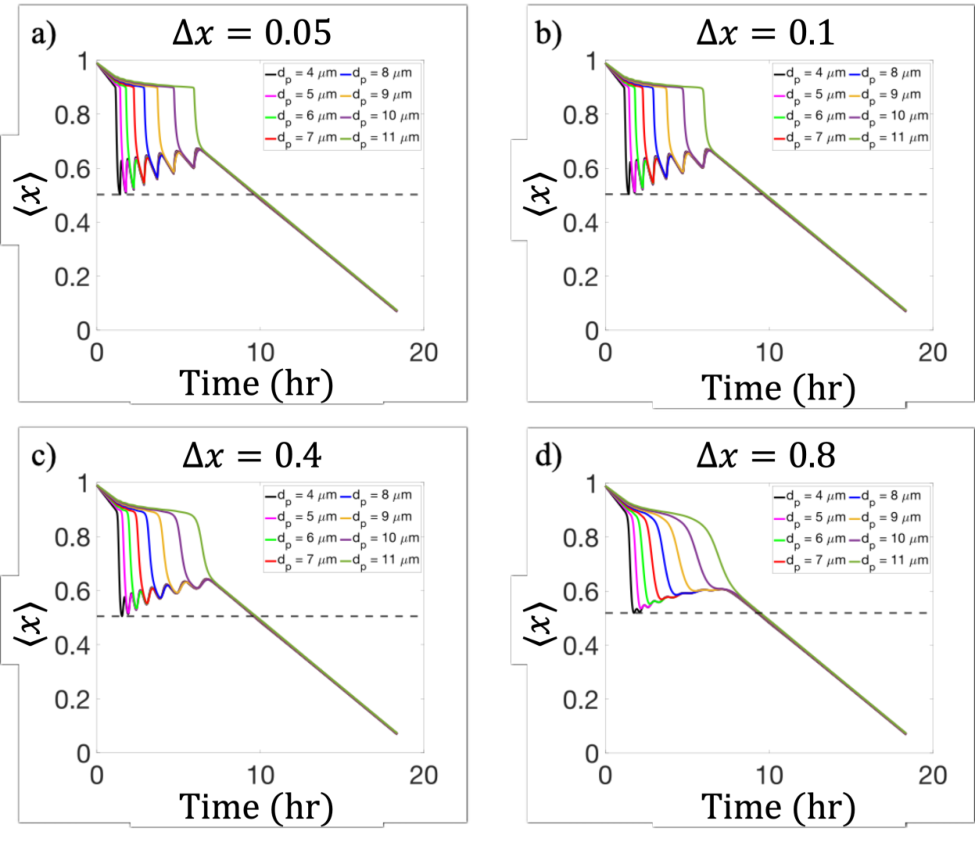
\includegraphics[width=\textwidth]{8-particle-evolution-deltax.pdf}
  \caption{Evolution of $\langle x\rangle$ for the
    8-particle system obtained using the model form of $i_0$ with
    four different values of $\Delta x$: a) 0.05, b) 0.1, c) 0.4, and d)
    0.8. The black dashed line in each plot represents
    $\langle x \rangle^\dag$ for the smallest particle in
    the ensemble. The rapid delithiation rate and the amplitude of
    the oscillations decrease as $\Delta x$ increases.}
  \label{fig:delta-x-sensitivity}
\end{figure}

\section{Additional Figures}

\begin{figure}
  \centering
  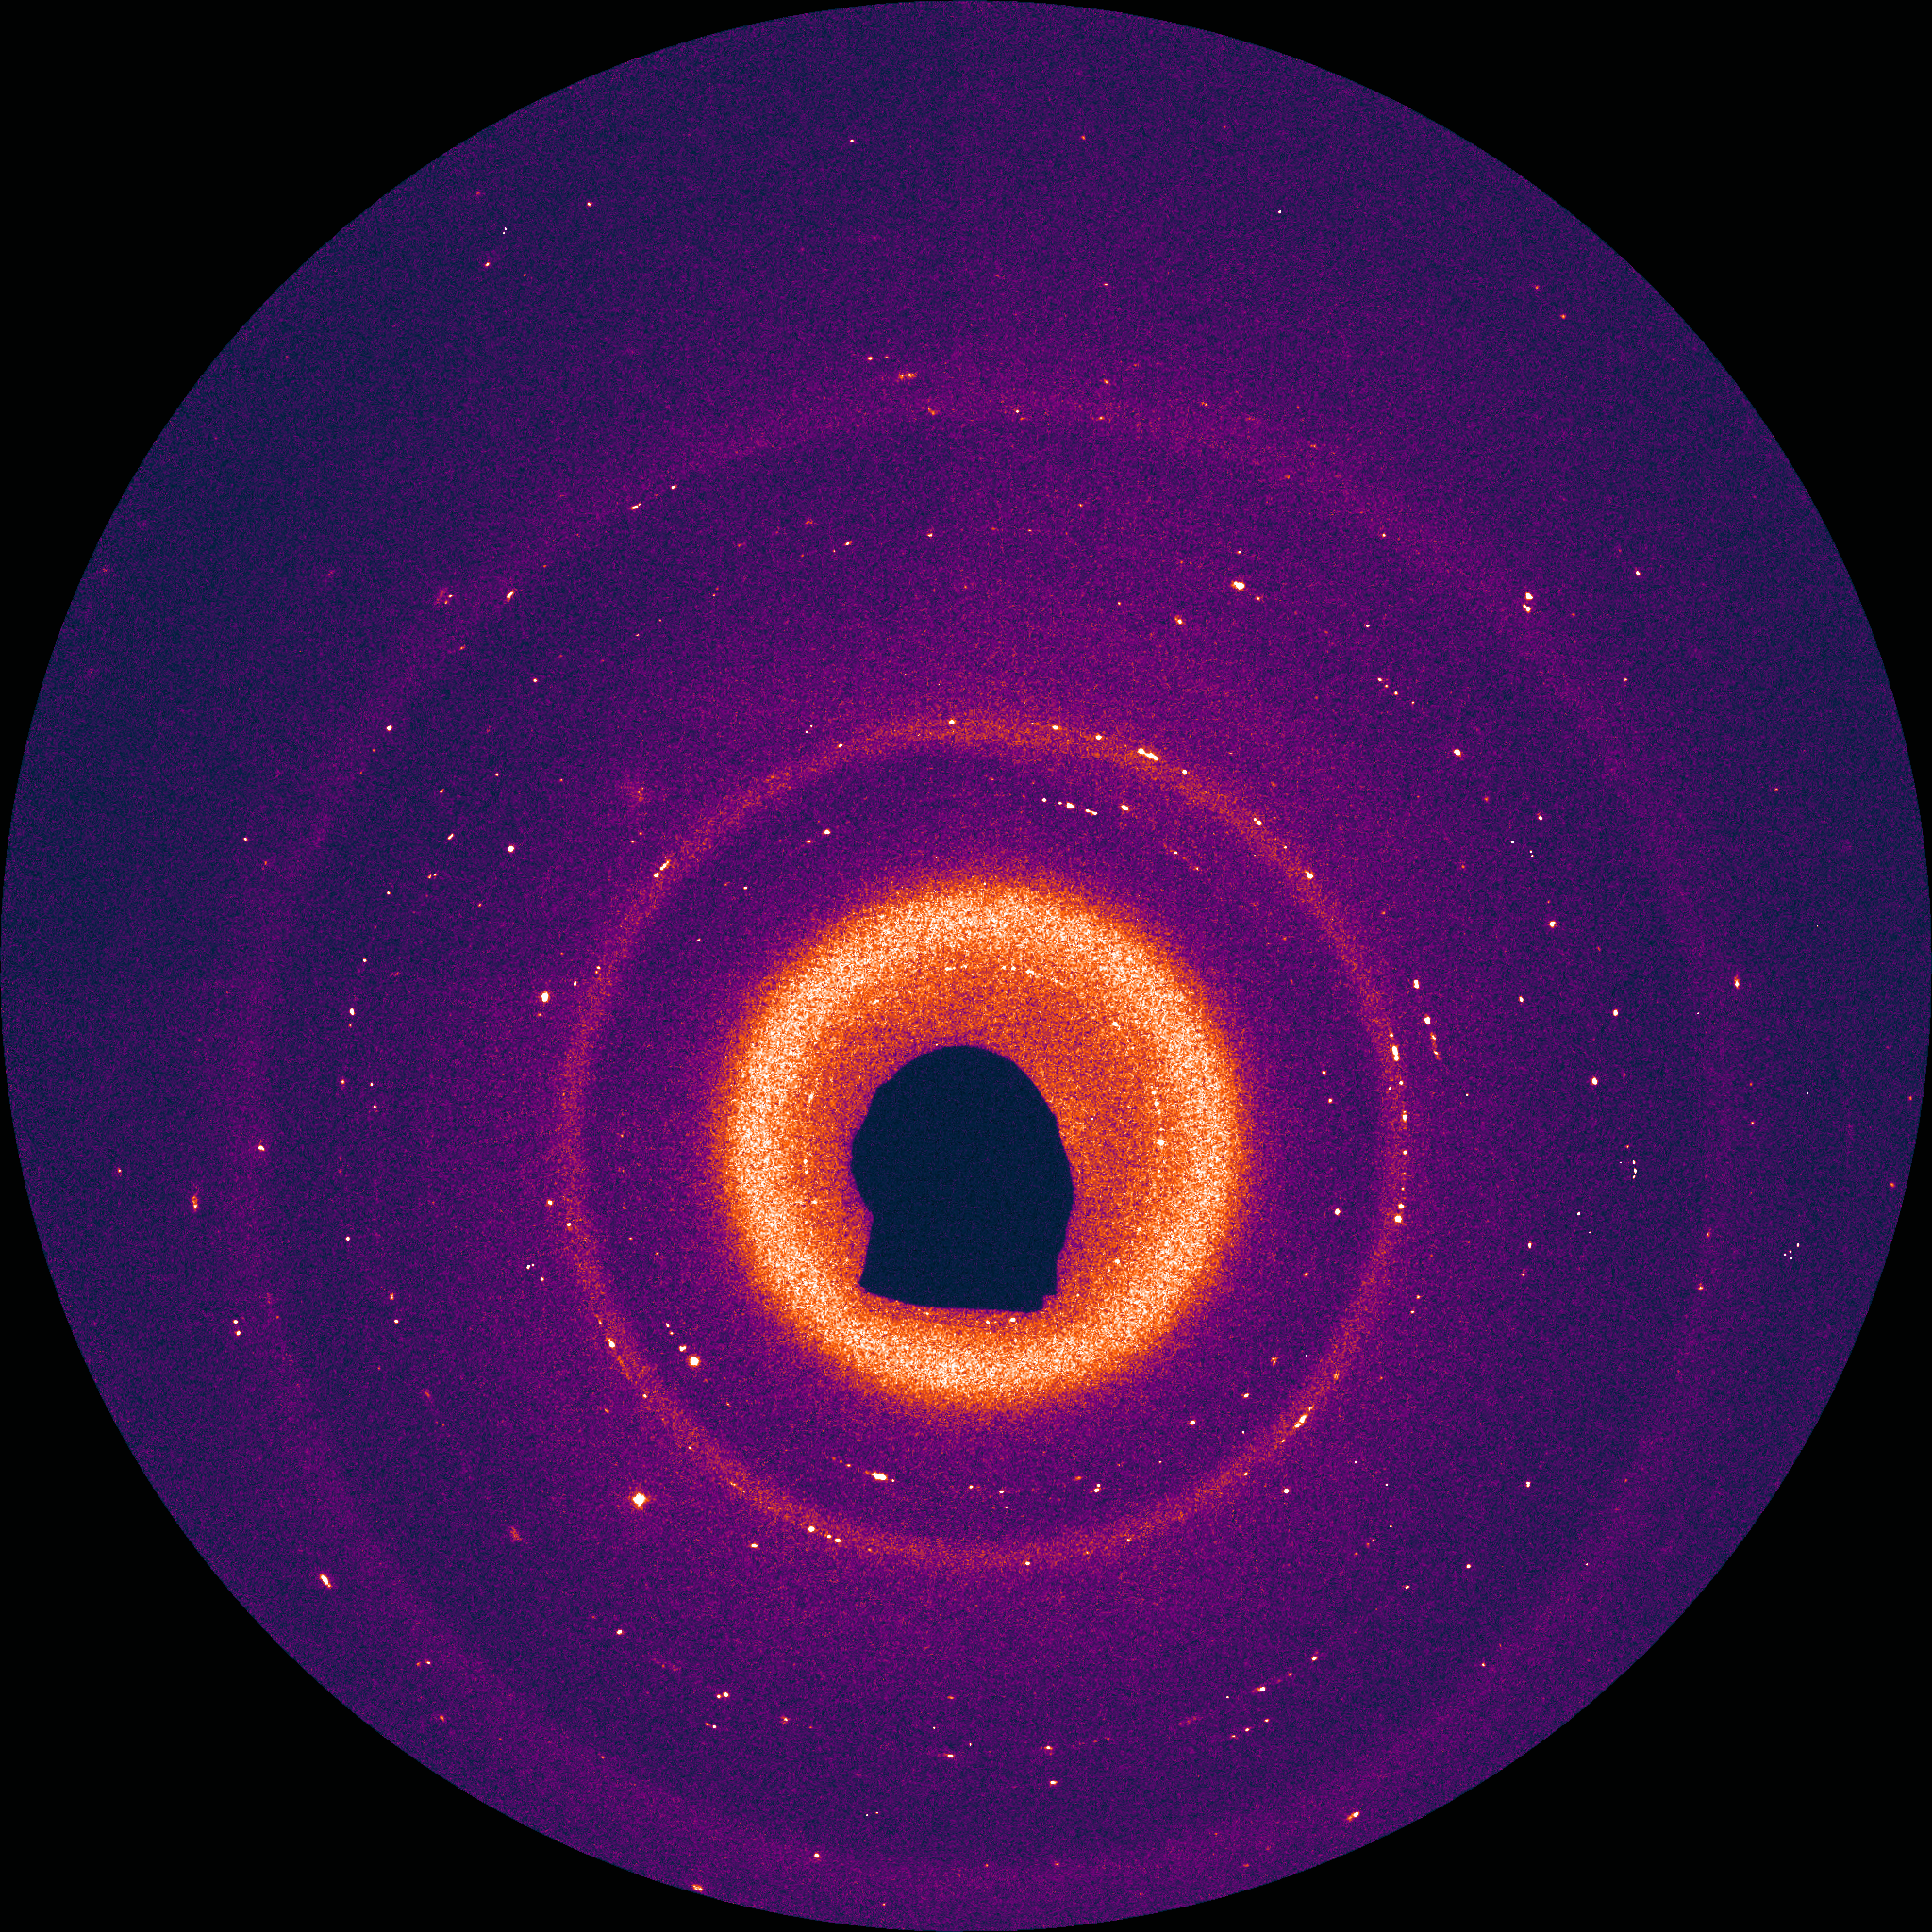
\includegraphics[width=0.5\linewidth]{figures/2D-diffraction.png}
  \caption{Exemplar 2D diffraction pattern for a single position
    during charging.}
  \label{fig:2Ddiffraction}
\end{figure}

\begin{figure}
  \centering
  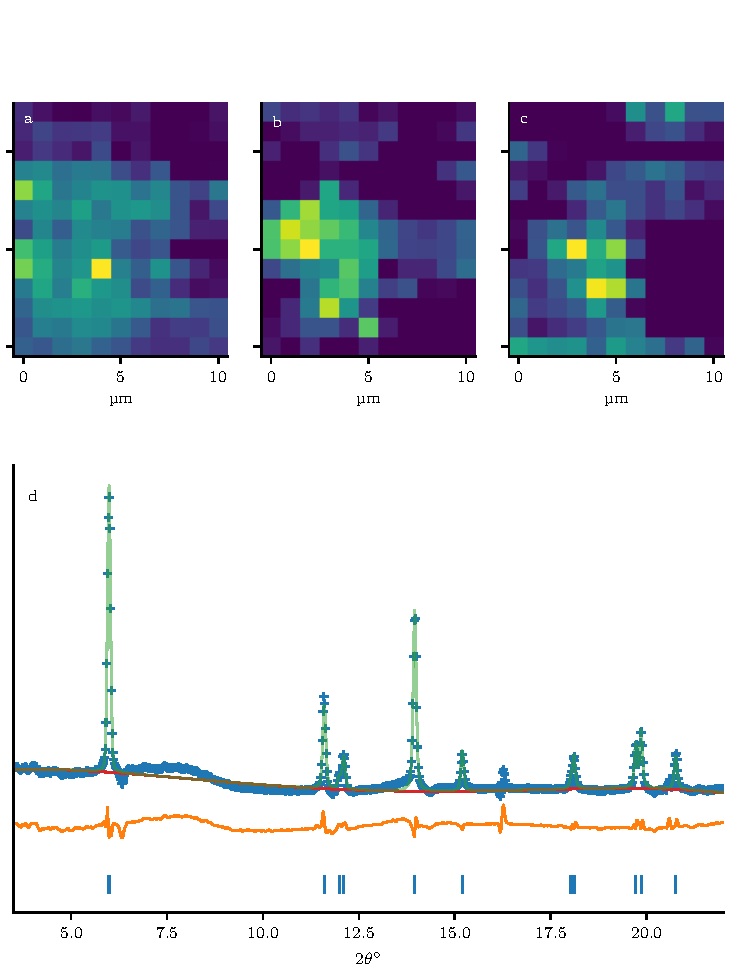
\includegraphics{figures/NCA-particles-refined.pdf}
  \caption{\nca{} \gls{uxrd}. (a-c) Maps of summed diffraction
    intensity for particles 1, 2, and 3 repsectively. (d-f)
    Whole-pattern LeBail refinements for summed diffraction intensities
    of particle 1 (d) in the pristine state, (e) during first charge,
    and (f) at the end of first charge. Ticks show expected positions
    for reflections of \nca{} with $\rm{R\bar{3}m}$ space group.}
  \label{fig:refinements}
\end{figure}

\begin{figure}
  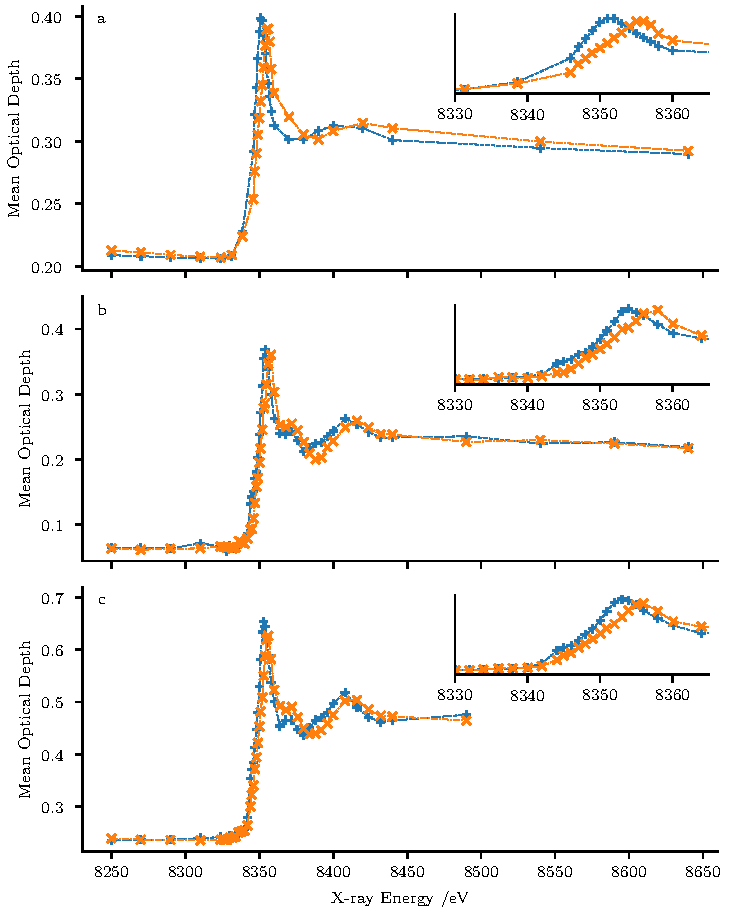
\includegraphics{figures/Kedges.pdf}
  \caption{Ni K-edge absorption spectra for TXM fields of view. Mean
    optical depth of pixels after edge filter for
    (\textcolor{C0}{\mplreduced{}}) most reduced and
    (\textcolor{C1}{\mploxidized{}}) most oxidized time-steps for (a)
    \nmc[333]{}, (b) \nca{}, and (c) \nmc[532]{}.}
  \label{fig:kedges}
\end{figure}

\begin{figure}
  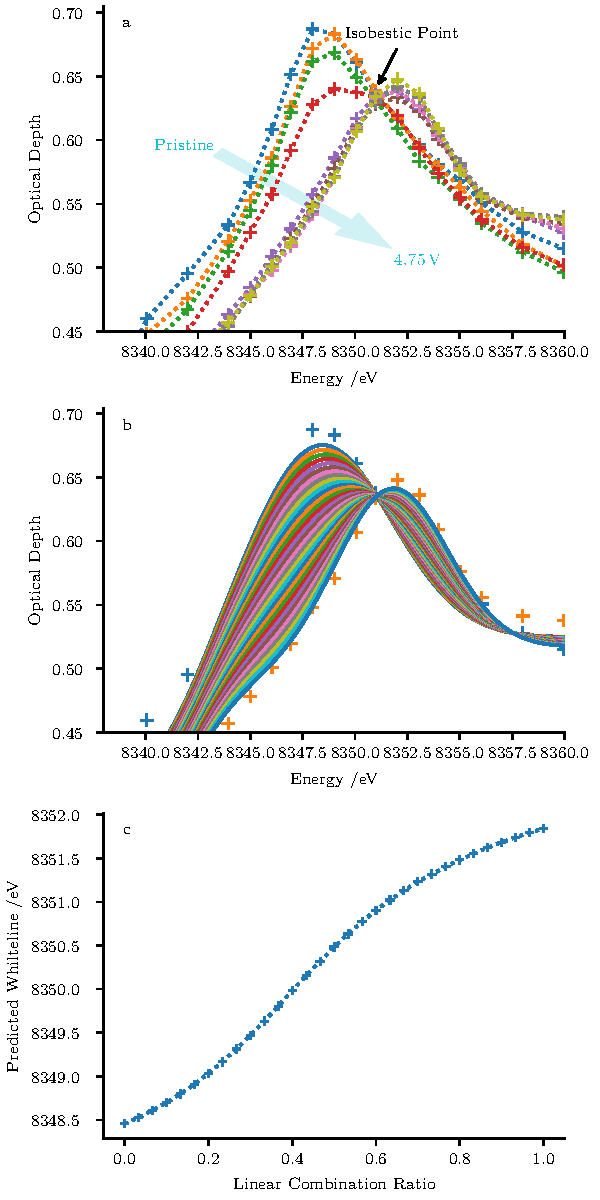
\includegraphics{figures/isobestic-point.pdf}
  \caption{Demonstration of isobestic point for \nmc[333]{} \ce{Ni}
    K-edge. (a) Observed mean optical depth spectra for \gls{txm}
    frames during operando oxidation, with dashed lines added as
    visual guides. (b) Results of mathematical linear combinations of
    fit spectra (\mplline{}) for observed spectral end-members for the
    most reduced (\textcolor{C0}{+}) and oxidized (\textcolor{C1}{+})
    points in the \nmc[333]{} frames in (a). (c) Effect of linear
    combination ratio of spectral end-members in \emph{b} on resultant
    whiteline energy.}
  \label{fig:isobestic-point}
\end{figure}

\begin{figure}
  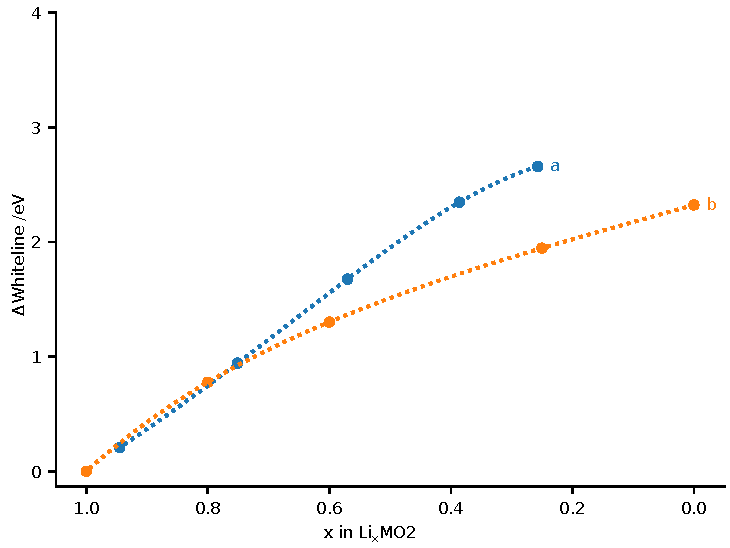
\includegraphics{figures/bulk-xas-extraction.pdf}
  \caption{Reported changes of \ce{Ni} K-edge whiteline energy. (a)
    In-situ XAS of \nmc[333]{x} and (b) ex-situ XAS of \nca{x}. Data
    extracted from published figures as described in Table
    \ref{tab:bulk-xas-extraction}.}
  \label{fig:bulk-xas-extraction}
\end{figure}

\begin{table}
  \begin{tabular}{c c c | c c c}
    \multicolumn{3}{c|}{\nmc[333]{x}} & \multicolumn{3}{c}{\nca{x}} \\
    x & Whiteline /eV & \textDelta{} /eV & x & Whiteline /eV & \textDelta{} /eV \\
    \hline\hline
    0.945 & 8353.98 & 0.21 & 1.00 & 8348.84 & 0.00 \\
    0.751 & 8354.72 & 0.94 & 0.80 & 8349.61 & 0.78 \\
    0.570 & 8355.45 & 1.68 & 0.60 & 8350.14 & 1.30 \\
    0.386 & 8356.12 & 2.35 & 0.25 & 8350.78 & 1.95 \\
    0.257 & 8356.43 & 2.66 & 0.00 & 8351.16 & 2.32 \\
  \end{tabular}
  \caption{Reported energies of \ce{Ni} K-edge whiteline. In-situ
    \gls{xas} of \nmc[333]{x} (Ref.\ \cite{deb2005}) and ex-situ
    \gls{xas} \nca{x} (Ref.\ \cite{muto2009}). Data extracted from
    published figures using
    WebPlotDigitizer\cite{webplotdigitizer}. Relative shifts in
    whiteline energy (\textDelta{}) calculated as difference from
    fully lithiated state ($x=1$).}
  \label{tab:bulk-xas-extraction}
\end{table}

\begin{figure}
  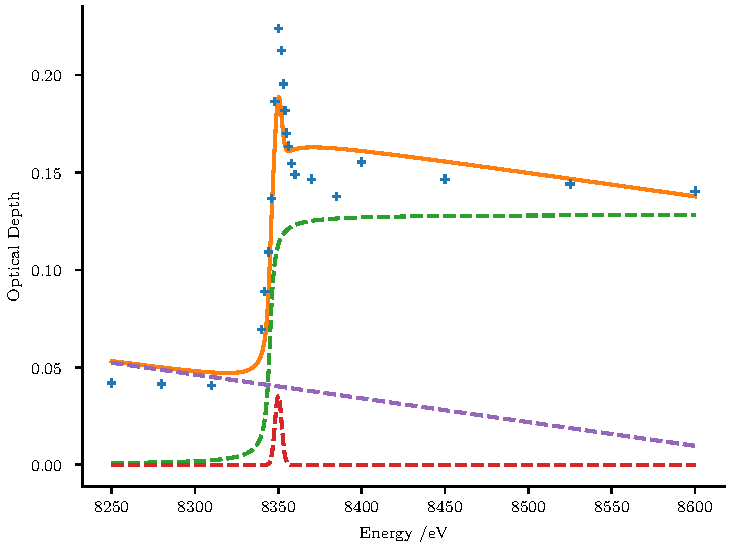
\includegraphics{figures/kedge-decomposition.pdf}
  \caption{Sample decomposition of Ni K-edge fitting. Spectrum of mean
    optical depth of a frame of \nca{} particles as
    (\textcolor{C0}{\textbf{+}}) observed optical depth;
    (\textcolor{C1}{\mplline{}}) overall least squares fit; and
    (\textcolor{C2}{\mpldashes{}}) arctangent,
    (\textcolor{C3}{\mpldashes{}}) Gaussian and
    (\textcolor{C4}{\mpldashes{}}) background components of least
    squares fit.}
  \label{fig:kedge-decomposition}
\end{figure}

\begin{figure}
  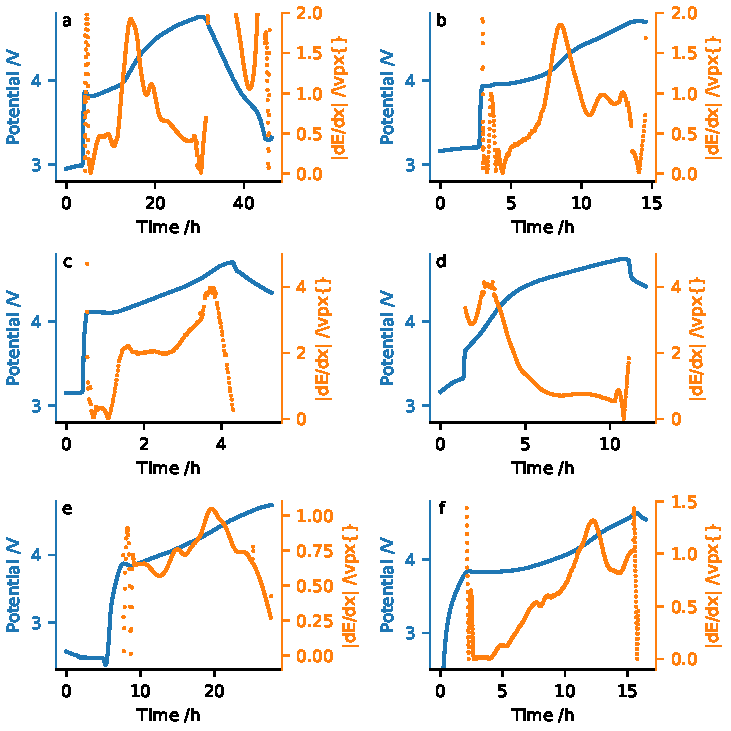
\includegraphics{figures/echem-derivatives.pdf}
  \caption{Cell potential (\textcolor{C0}{\mplline{}}) and derivative
    of potential with respect to $x$ in \ce{Li_xMO2}
    (\textcolor{C1}{\mpldots}) during galvanostatic
    charge/discharge. (a,b) \nmc[333]{} cathode in modified coin-cell
    during first charge, (c) \nca{} cathode in pouch-cell during first
    charge, (d) \nca{} cathode in pouch-cell during second charge, (e)
    \nca{} cathode charged in modified coin-cell, and (f) \nmc[532]{}
    cathode charged in modified coin-cell. All galvanostatic profiles
    treated with third-order Sovitzky-Golay filter with 101-point
    window prior to calculating derivative.}
  \label{fig:echem-derivatives}
\end{figure}

\begin{figure}
  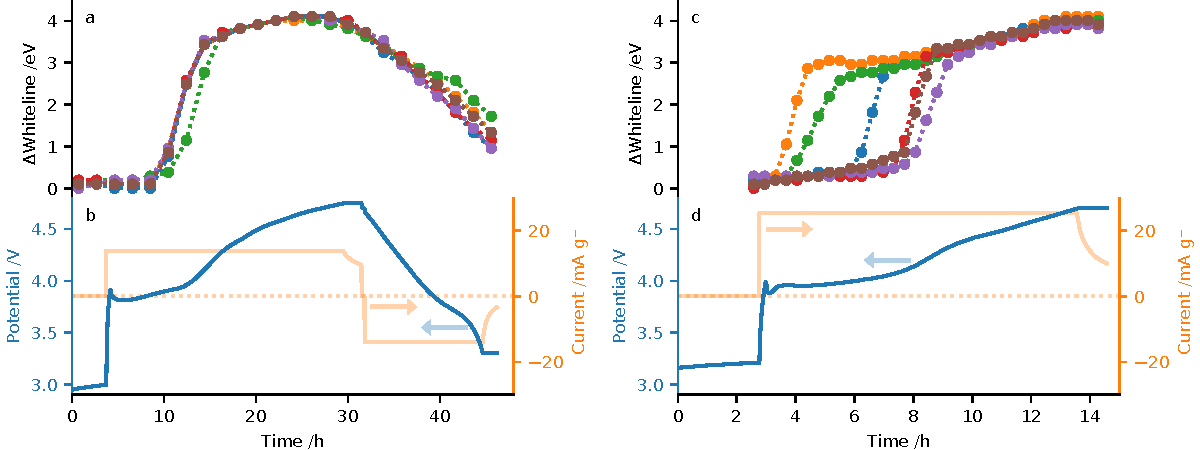
\includegraphics[width=\textwidth]{figures/NMC333-particle-echem.pdf}
  \caption{Particle-level oxidation during first charge and discharge
    of \nmc[333]{}. (a) Changes in mean whiteline energies relative to
    \SI{8351.69}{eV} for secondary particles during first charge and
    discharge. (c) Changes in mean whiteline energies relative to
    \SI{8351.22}{eV} for secondary particles with higher temporal
    resolution. (b,d) Operando potential (\textcolor{C0}{\mplline{}})
    and current (\textcolor{C1}{\mplline{}}) for galvanostatic cycling
    with \SI{4.75}{V} potentiostatic step for \nmc[333]{} samples in
    modified coin-cells.}
  \label{fig:nmc333-particles}
\end{figure}

\begin{figure}
  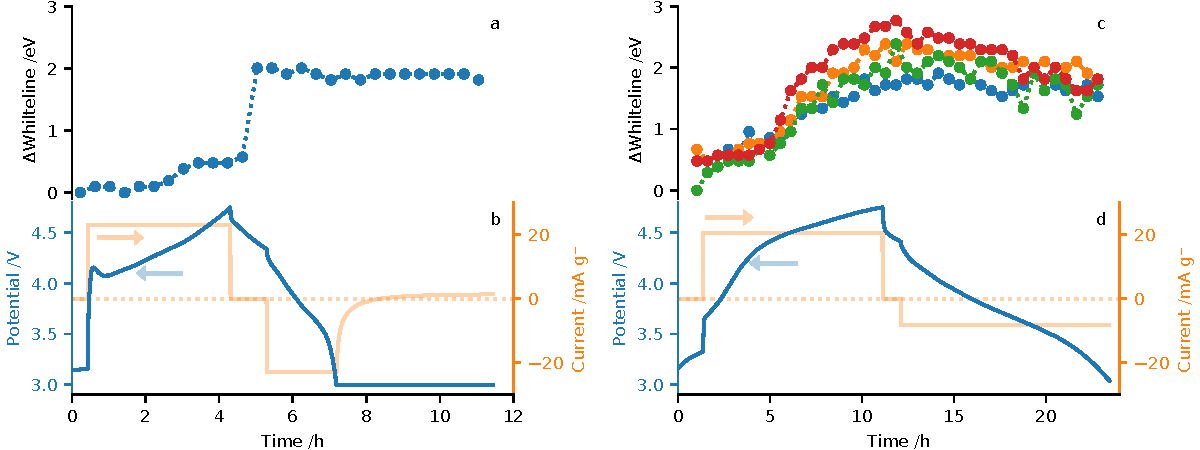
\includegraphics[width=\textwidth]{figures/NCA-particle-echem.pdf}
  \caption{Particle-level oxidation during first and second discharge
    of \nca{} samples in pouch cells. (a) Changes in mean whiteline
    energies relative to \SI{8350.92}{eV} for secondary particle
    during first charge/discharge cycle. (c) Changes in mean whiteline
    energies relative to \SI{8350.45}{eV} for secondary particles
    during second charge and discharge cycle. (b) Operando potential
    (\textcolor{C0}{\mplline{}}) and current
    (\textcolor{C1}{\mplline{}}) for galvanostatic oxidation,
    open-circuit potential, galvanostatic reduction, and
    potentiostatic reduction during first cycle. (d) Operando
    potential (\textcolor{C0}{\mplline{}}) and current
    (\textcolor{C1}{\mplline{}}) for galvanostatic oxidation,
    potentiostatic oxidation, and galvanostatic reduction during
    second cycle.}
  \label{fig:nca-particles}
\end{figure}

\begin{figure}
  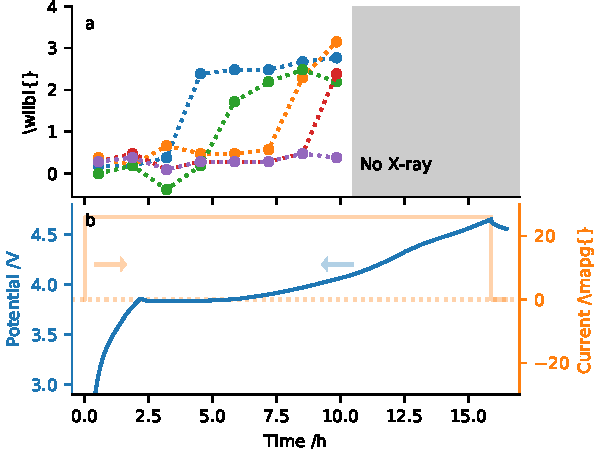
\includegraphics{figures/NMC532-particle-echem.pdf}
  \caption{Particle-level oxidation during first charge and discharge
    of \nmc[532]{}. (a) Mean whiteline energies of secondary particles
    during charge discharge. (b) Operando potential
    (\textcolor{C0}{\mplline{}}) and current
    (\textcolor{C1}{\mplline{}}) for galvanostatic cycling for
    \nmc[532]{} samples in modified coin-cells. X-rays unavailable
    after \SI{10}{\hour} due to maintenance.}
  \label{fig:nmc532-particles}
\end{figure}

\begin{figure}
  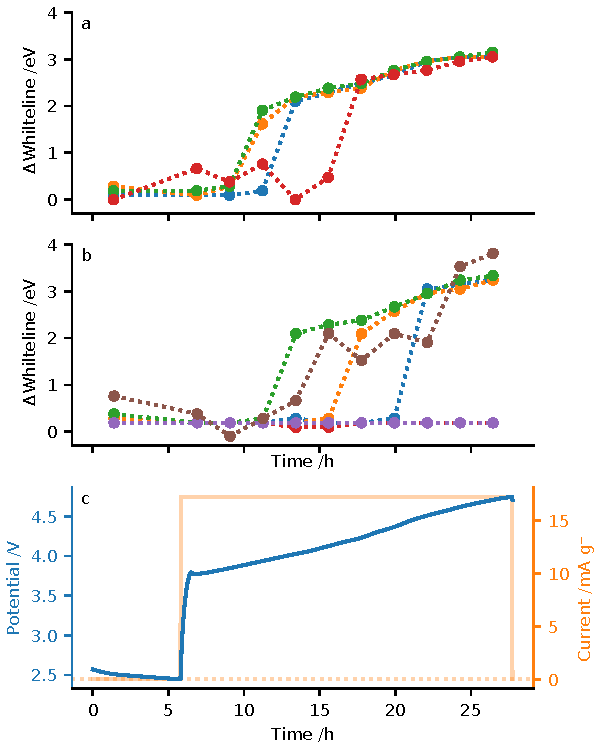
\includegraphics{figures/NCA-particles-irradiation.pdf}
  \caption{Operando \gls{txm} of secondary \nca{} particles during
    first charge. Mean changes in whiteline energies relative to
    \SI{8354.18}{eV} for secondary particles (a) without static X-ray
    exposure, and (b) with a \SI{3}{\hour} static X-ray exposure prior
    to operando imaging. (c) Galvanostatic charging profile for
    modified coin-cell with \nca{} cathode.}
  \label{fig:nca-irradiation}
\end{figure}


\begin{figure}
\centering   
  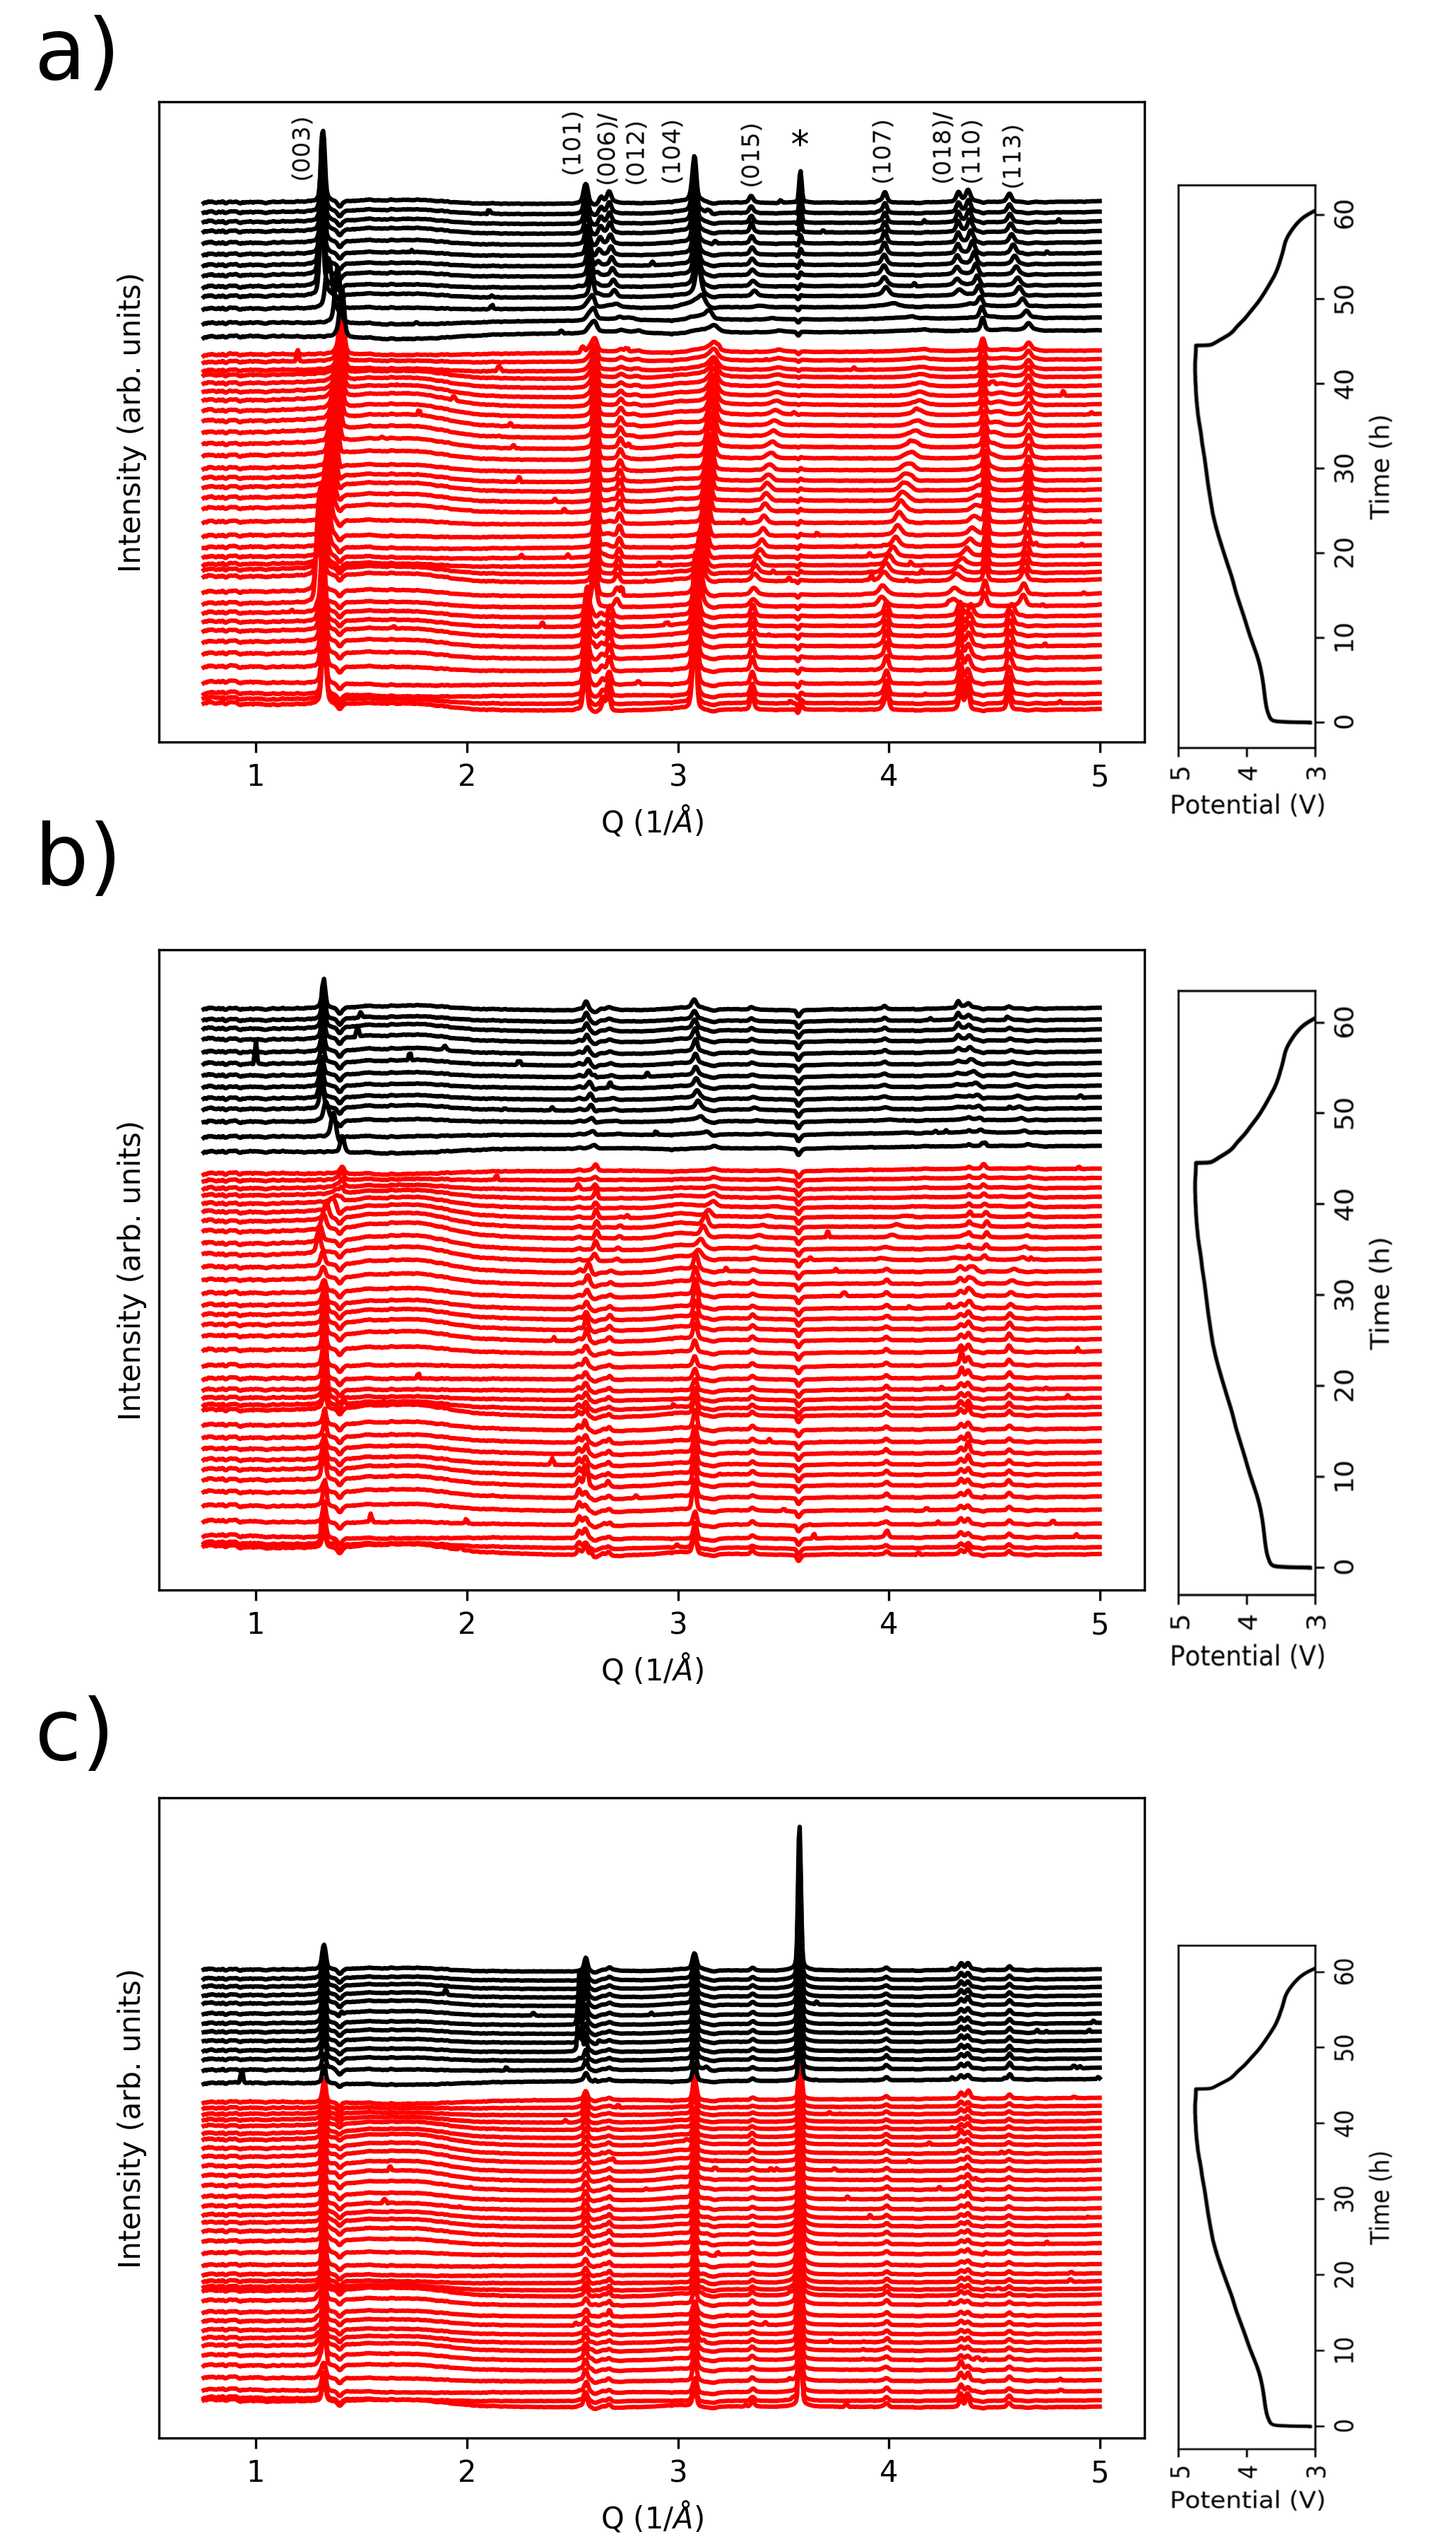
\includegraphics[width=\linewidth, height=0.8\textheight, keepaspectratio]{figures/p1-3-xrd.png}
  \caption{Diffraction patterns for \nca{} through charge (red) and
    discharge (black) for a) P1, b) P2, and c) P3. Feature due to
    \ce{Li} is denoted with a *.}
  \label{fig:xrd-echem}
\end{figure}

\begin{figure}
  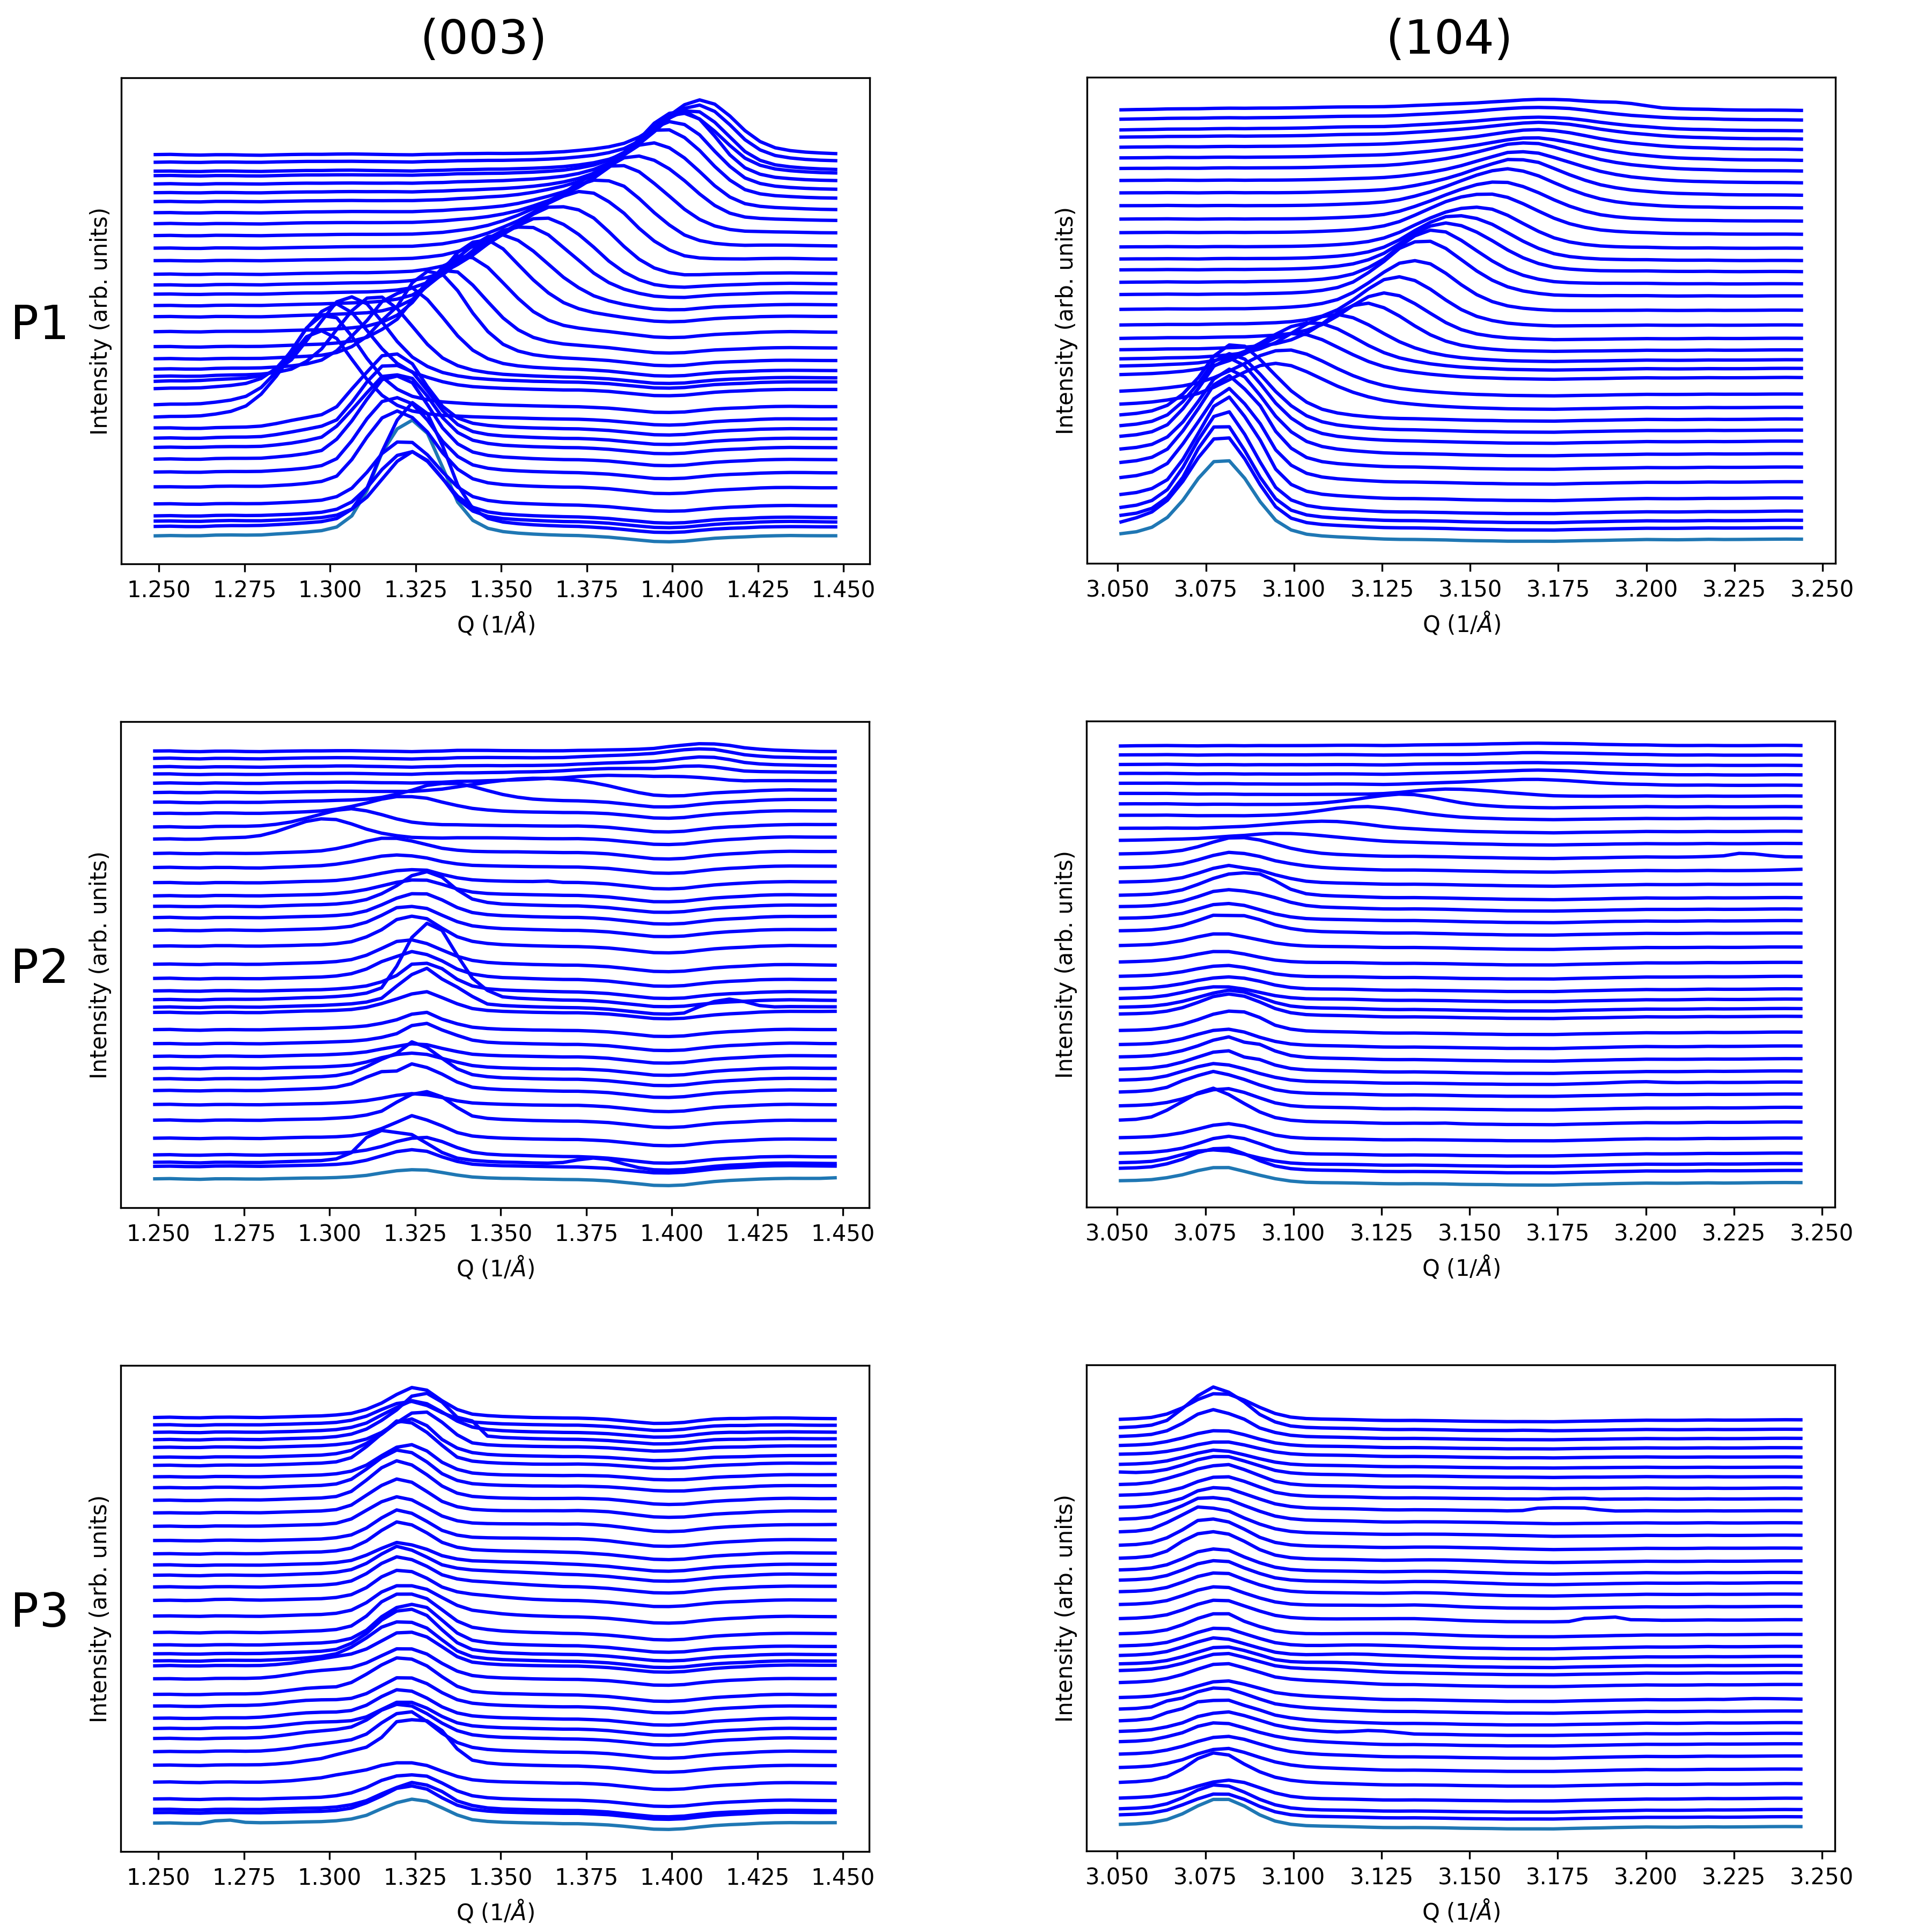
\includegraphics[width=\linewidth]{figures/ind-peaks.png}
  \caption{(003) (left) and (104) (right) reflections of P1, P2, and P3
    (top to bottom) during the first charge.}
  \label{fig:ind-peaks}
\end{figure}


\begin{figure}
  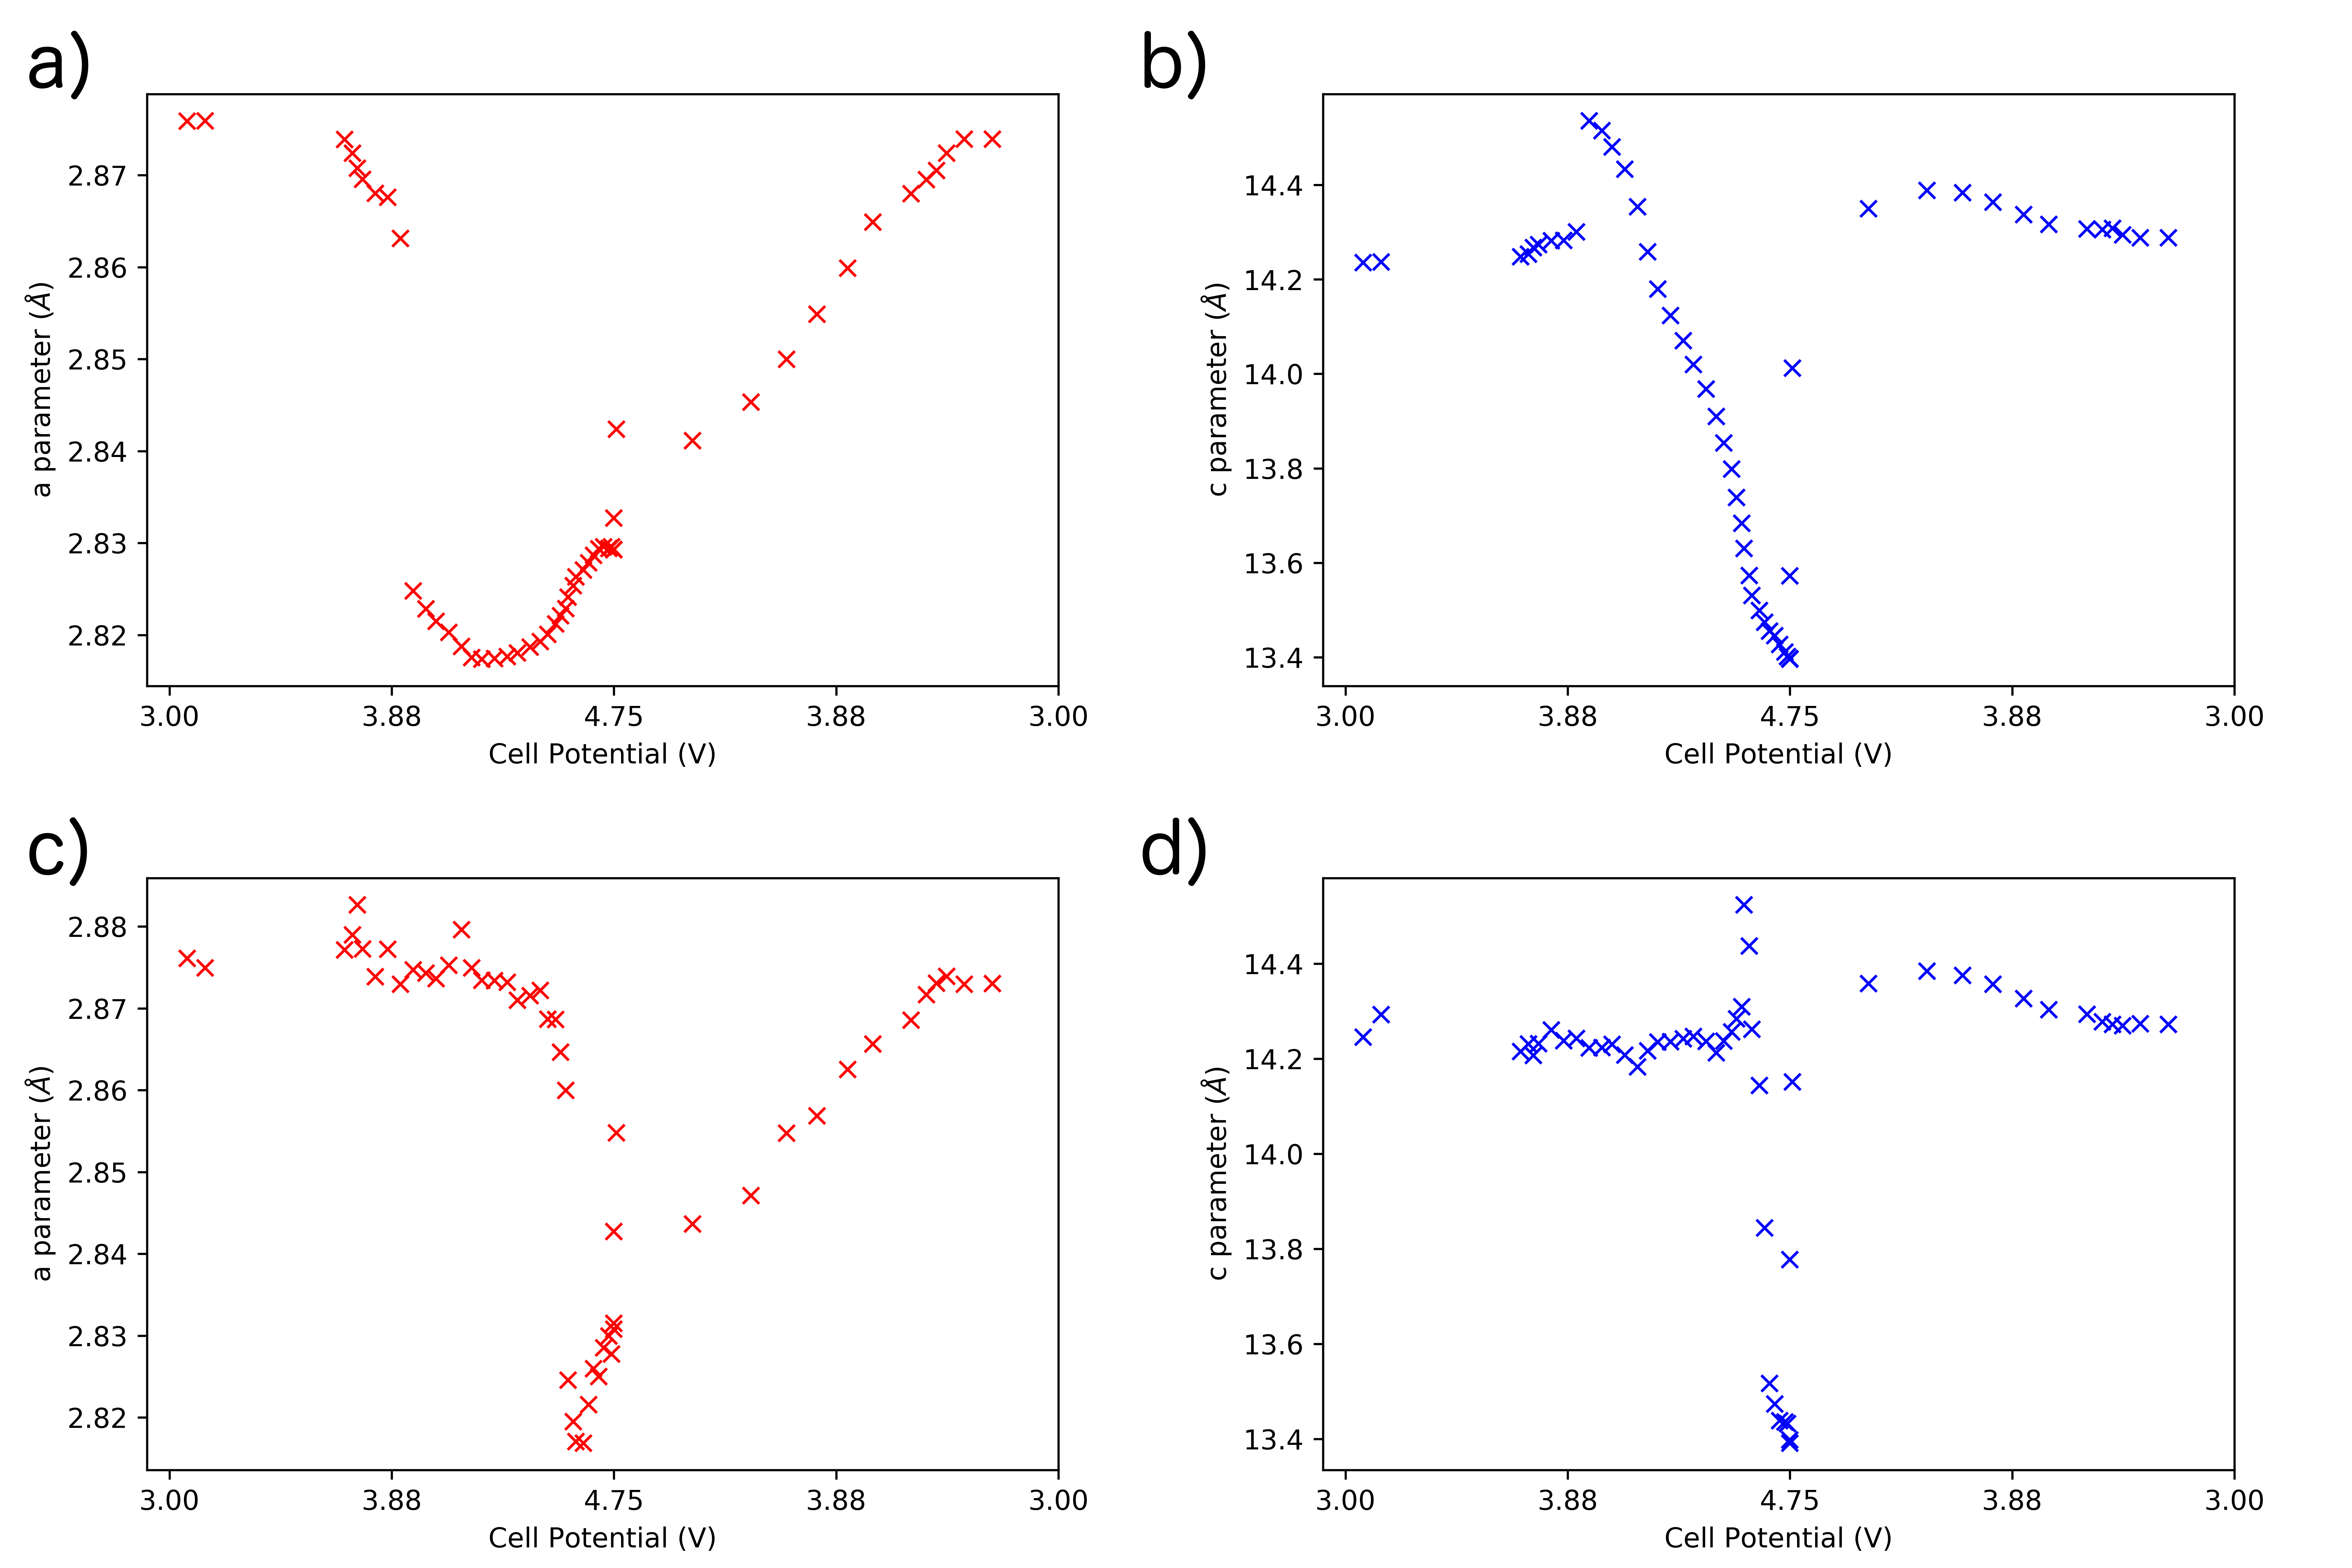
\includegraphics[width=\linewidth]{figures/cell-pars.png}
  \caption{Unit cell parameters as a function of cell potential for a)
  P1 a parameter b) P1 c parameter c) P2 a parameter and d) P2 c parameter}
  \label{fig:cell-pars}
\end{figure}

\begin{figure}
  \centering
  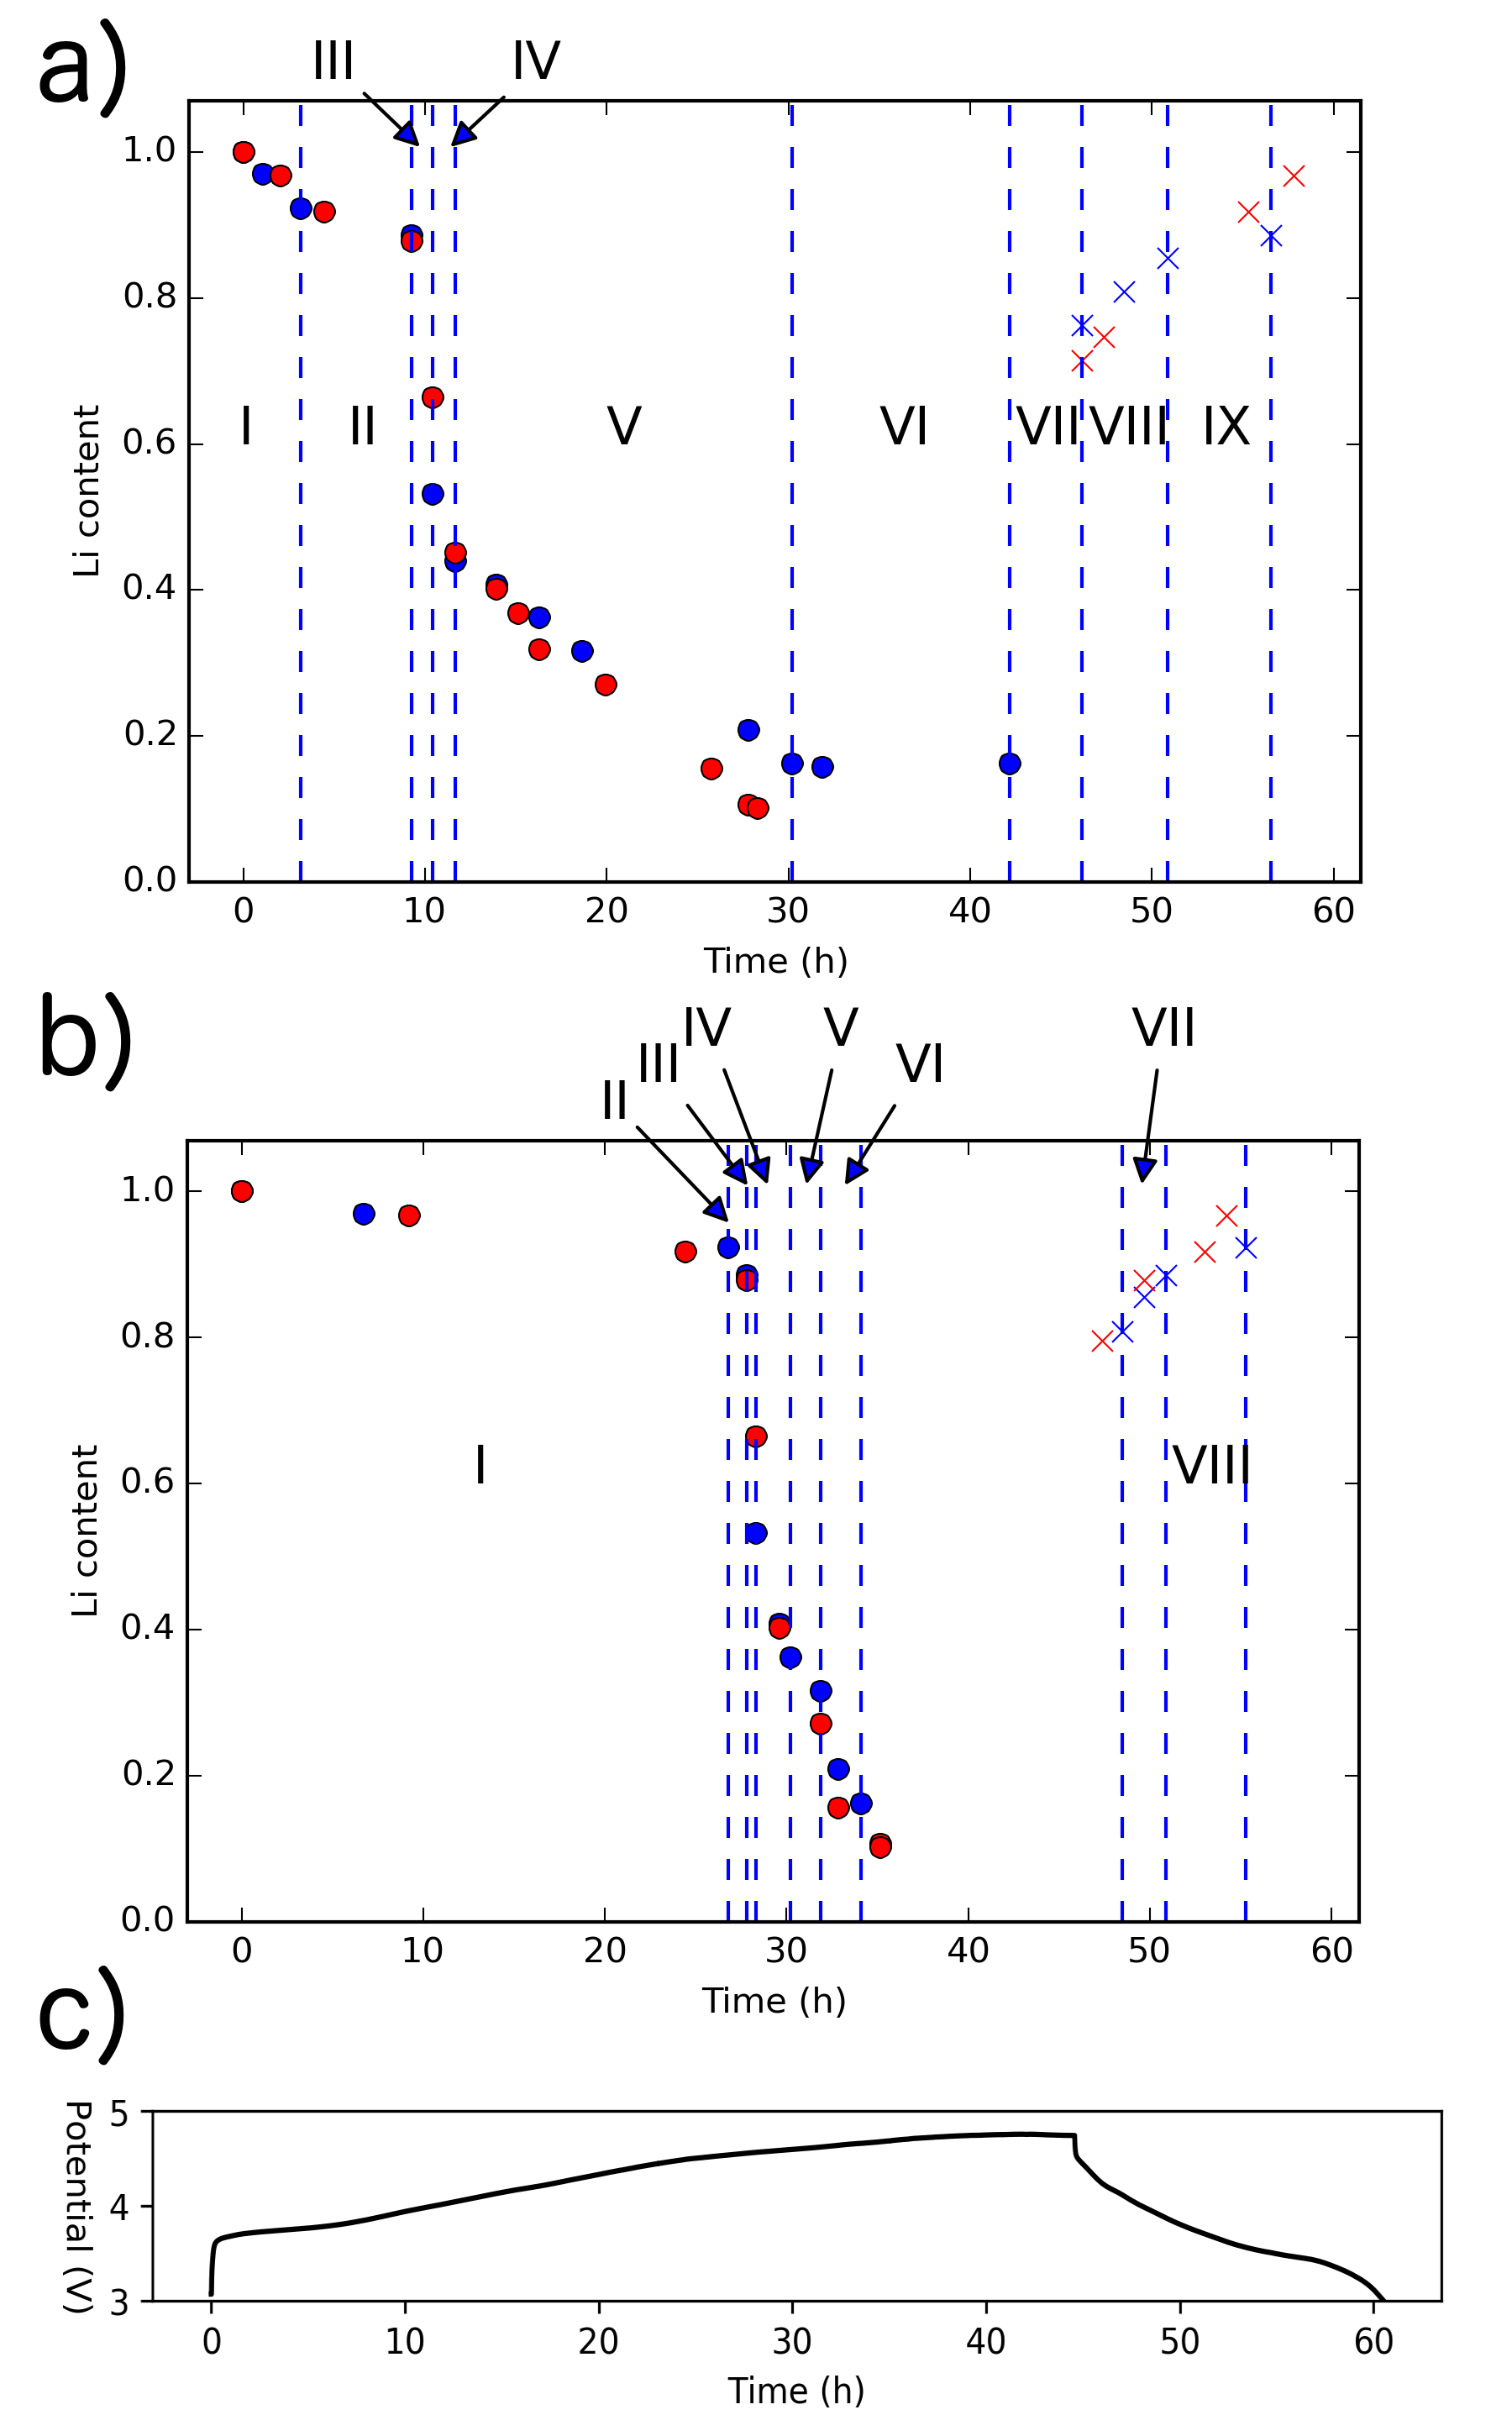
\includegraphics[width=\linewidth, height=0.8\textheight,keepaspectratio]{figures/rate-plots.png}
  \caption{\ce{Li} content (x in
    \ce{Li_xNi_{0.80}Co_{0.15}Al_{0.05}O2}) as a function of time
    during the first cycle for P1 (a) and P2 (b). The charge-discharge
    curve is shown below (c). \ce{Li} values were correlated with
    equivalent values in ref. \cite{robert2015}, for the a unit cell
    parameter (red) and c unit cell parameter (blue). Charge is
    represented by circles while discharge is represented by x
    markers.}
  \label{fig:rates}
\end{figure}

\clearpage
\pagebreak

\bibliographystyle{plain}
\bibliography{refs,refs-extra}

\end{document}
